% The line below matches the stock Springer Nature template: single spacing, no
% line numbers. Journal of Big Data asks the file uploaded to the editorial
% system to carry double-line spacing and line numbering; the class supplies both
% as options, and neither is enabled here by author preference.
%
%   referee -> global \doublespacing (setspace). It applies to body text, tables
%              and captions alike; the class's \singlespacing under \if@referee
%              touches only the article-category box on the front page.
%   lineno  -> line numbers in the margin, via the class's own vruler.
%
% To produce the submission file, add them back:
%   \documentclass[sn-vancouver,Numbered,referee,lineno]{sn-jnl}
\documentclass[sn-vancouver,Numbered]{sn-jnl}

% sn-jnl.cls expects these two to be present in the document preamble.
\usepackage{manyfoot}
\usepackage{xcolor}
\definecolor{artcatboxgray}{gray}{0.94}

\usepackage{graphicx}
\usepackage{multirow}
\usepackage{amsmath}
\usepackage{amssymb}
\usepackage{amsfonts}
\usepackage{booktabs}
\usepackage{array}
\usepackage{url}

\raggedbottom

\newcommand{\vr}{\rule{0pt}{2.4ex}}

\begin{document}

\title[Auditable Temporal Machine Learning for Prosecutorial Workload]{Auditable temporal machine learning for prosecutorial workload: a framework for availability control, predictive assessment and decision utility in open administrative records}

% ORCID iDs are attached to the author records in the editorial system, which is
% how Springer Nature collects them; they are recorded here for reference.
%   M. Evangelista Gamarra -- https://orcid.org/0009-0002-5382-1390
%   J. A. Chancan Labajos  -- TODO(submission): register an ORCID iD and add it here.
\author*[1]{\fnm{Mois\'es} \sur{Evangelista Gamarra}}\email{mevangelistag@senati.pe}

\author[1]{\fnm{Jerremi Aron} \sur{Chancan Labajos}}\email{152048@senati.pe}

\affil*[1]{\orgname{Servicio Nacional de Adiestramiento en Trabajo Industrial (SENATI)}, \city{Lima}, \country{Peru}}

\abstract{Operational overload in prosecution services can hinder timely case processing and complicate the allocation of institutional capacity. This study develops and evaluates a reproducible temporal machine learning framework for predicting an operational-overload proxy from open administrative records of the Peruvian Public Prosecutor's Office, covering 9{,}593 operational unit-years from 2019 to 2026. The methodological contribution is an auditable protocol that makes four aspects explicit: when each predictor becomes available, which role each temporal partition is allowed to play, how predictor selection is constrained to the earliest training information, and whether predictive discrimination is consistent with calibration and decision utility. Candidate predictors are classified as ex ante, concurrent or ex post, and the availability audit is repeated against the feature matrix that is actually fitted. This second audit exposed three publication-metadata indicators that survived feature selection; they are retained and reported as a residual methodological exposure rather than being concealed. The temporal protocol uses 2019--2023 for model development, 2024 for operating-threshold selection and conformal calibration, 2025 as a single locked evaluation set, and the partial 2026 file as an exploratory temporal generalization check. On the locked 2025 evaluation, the reported XGBoost configuration attains a ROC-AUC of 0.796 (95\% CI 0.760--0.838), a PR-AUC of 0.400 and an F1-score of 0.409 at the operating threshold selected on 2024. Calibration analysis shows systematic over-estimation at higher predicted scores, while decision-curve analysis indicates negative net benefit at the F1-optimal threshold. These findings indicate that discrimination alone is insufficient to establish operational readiness. The framework is therefore presented as an auditable ranking and review-prioritisation procedure rather than as an automated alerting system, and the remaining requirements for deployment are explicitly identified.}

\keywords{judicial analytics, prosecutorial workload, data leakage, model calibration, decision curve analysis, explainable machine learning, open government data}

\maketitle

\section{Introduction}\label{sec:intro}

Prosecution services are the entry point of the criminal justice chain, and the volume of files that accumulate at that entry point conditions everything downstream. When incoming cases persistently exceed processing capacity for a given territory, subject matter and case type, the resulting backlog lengthens response times, erodes procedural guarantees and makes the planning of human and budgetary resources reactive rather than anticipatory. Administrative registries published under open data mandates now make this imbalance measurable at national scale, and the natural question is whether the imbalance of a coming year can be anticipated from what is already known when that year begins.

Machine learning is an obvious candidate for that question, and a growing literature applies it to judicial workload, procedural duration and institutional performance. Much of that literature, however, evaluates its components in isolation: a feature selection strategy is benchmarked without an accompanying leakage audit, a temporal validation scheme is proposed without a calibration assessment, or an interpretability method is observed without asking whether the resulting scores would support a decision at all. The consequence is a body of reported performance figures whose operational meaning is difficult to establish, because the reader cannot tell which information the model actually had access to at the moment the prediction is supposed to be issued, nor whether the predicted probabilities mean what their scale suggests.

This paper addresses that gap for the prosecutorial domain, and it does so by treating three questions that are usually left implicit as first-class methodological objects.

\emph{What information can the model legitimately know at prediction time?} We define an explicit prediction time point and classify every candidate predictor as ex ante, concurrent or ex post. Concurrent and ex post variables are excluded from the intended predictor set, including the volumetric variables that construct the proxy label. The availability audit is then repeated against the feature matrix produced by the selection stage. This distinction is essential because a variable can be inadmissible in principle yet re-enter the fitted matrix through downstream feature engineering or selection. The framework therefore treats availability verification as an auditable property of the final feature matrix rather than as an assumption derived from the initial exclusion rule.

\emph{Which role does each temporal partition play?} Each partition is assigned a pre-specified and explicitly documented function. The training block is used for model development, 2024 is reserved for operating-threshold selection and conformal calibration, 2025 remains locked for final evaluation, and the partial 2026 file is treated only as an exploratory temporal generalization check. This separation prevents the final evaluation from being used to optimise an operating decision.

\emph{Is the resulting score useful, and at what price?} We separate discrimination from calibration and from decision-analytic utility, and we report the direction as well as the magnitude of calibration error. Where the evidence does not support a claim of operational usefulness, we say so and characterise the conditions under which it would.

The methodological contributions of this work are therefore fivefold. First, we formalise a temporal availability audit that classifies candidate predictors according to when they become observable and requires the classification to be verified again against the feature matrix that is actually fitted. Second, we define a temporal partition protocol that separates model development, operating-point selection, final evaluation and exploratory temporal generalisation. Third, we constrain consensus feature selection to the earliest training information and combine six complementary selection procedures to reduce dependence on any single selector. Fourth, we integrate discrimination, calibration, decision-curve analysis, subgroup performance, temporal drift and conformal uncertainty into a single audit-oriented evaluation rather than treating predictive accuracy as effective evidence for deployment. Fifth, we provide the availability-audit template and reproducible implementation as reusable methodological artefacts for longitudinal administrative registries. The empirical case is prosecutorial workload in Peru; the transferable contribution is the audit protocol.

A word on scope is in order. The empirical registry is national but modest in size, and the study is not intended to claim a universally optimal predictive model for prosecutorial workload. The contribution is methodological: the registry serves as a demanding case study in which temporal availability, derived administrative variables, periodic publication metadata, class imbalance and temporal distribution shift can interact. The framework is therefore presented as a reusable procedure for longitudinal administrative registries, while transferability beyond the present registry remains an empirical question. The availability audit is supplied as a reusable template rather than only as a study-specific result.

Section~\ref{sec:related} reviews the relevant literature. Section~\ref{sec:methods} describes the data, the availability audit, the partition protocol and the modelling pipeline. Section~\ref{sec:results} reports the results, Section~\ref{sec:discussion} interprets them, and Sections~\ref{sec:limits} and~\ref{sec:conclusions} state the limitations and conclusions.

\section{Related work}\label{sec:related}

\subsection{Predicting judicial and prosecutorial workload}

Research on the quantitative modelling of case flow has concentrated on the judicial phase of the process. Studies have combined tree-based learners with attribution methods to model case duration and congestion \cite{azaria_alleviating_2024}, applied process mining and temporal analysis to identify procedural bottlenecks and measure institutional throughput \cite{pernici_improving_2024}, and analysed court productivity from administrative registries \cite{vasconcelos_analysis_2023}. Review work documents a shift away from isolated predictive exercises and towards integrated frameworks for the management of justice systems \cite{hannoon_artificial_2025}.

Two features of this literature motivate the present study. The first is scope: the prosecutorial stage that precedes judicial proceedings receives markedly less attention than the judicial stage itself, even though it determines the volume that reaches the courts. The second is protocol: reported evaluations rarely state which information was available at the moment the prediction is nominally issued, which makes it difficult to judge whether the performance figures could survive deployment. Our contribution is directed at the second point as much as the first.

\subsection{Feature selection under correlated predictors}

Feature selection influences the stability, interpretability and generalisation of a classifier. Filter methods score predictors independently of any learner and are cheap but blind to interactions; wrapper methods exploit the predictive performance of a specific classifier at substantially higher computational cost \cite{zhou_efficient_2024}; embedded methods perform selection during training but inherit the inductive bias of the chosen algorithm. Because individual selectors disagree in the presence of correlated predictors, and because that disagreement produces unstable feature subsets, ensemble and consensus strategies have been proposed to aggregate several criteria into a more stable decision \cite{zhou_efficient_2024,moslemi_tutorial-based_2023}. Among embedded all-relevant selectors, the Boruta algorithm compares the importance of each predictor against randomised shadow copies within a Random Forest, providing a statistical relevance test rather than a minimal-optimal subset \cite{kursa_feature_2010}.

The framework presented here follows that consensus logic, using six complementary selectors and a stability score, and preceding them with an explicit multicollinearity audit. What we add is a constraint on \emph{when} the selection may look at the data: the selectors are fitted only on the earliest training block and checked on a later, still-internal year, so that selection itself cannot borrow information from the evaluation period.

\subsection{Leakage, temporal validation and class imbalance}

Data leakage is a documented and widespread failure mode. A systematic review has traced overestimated performance across hundreds of studies in several disciplines to a small number of recurring patterns, chief among them computing preprocessing statistics over the full data set before partitioning \cite{kapoor_leakage_2023}. Restricting all preprocessing to the training partition and validating along the time axis are the standard remedies \cite{kapoor_leakage_2023,sasse_leakage_2023}, and leakage-free evaluation protocols have been proposed as a default practice \cite{hamdan_julearn_2023}.

We adopt those remedies, and extend them in one direction that the leakage literature treats less often. Beyond preprocessing leakage, an administrative data set carries variables that are perfectly legitimate as descriptors of a closed record but unavailable at prediction time --- publication dates, file-provenance identifiers, and any quantity computed from the outcome year itself. A model that uses them will validate cleanly under a temporal split and still be undeployable. Making that distinction explicit, variable by variable, is one of the contributions of this paper.

On class imbalance, synthetic minority oversampling \cite{chawla_smote_2002} is a common response. We do not use it: at an observed imbalance close to 85/15, cost-sensitive class weighting is effective and avoids introducing interpolated records into a registry whose rows correspond to real administrative aggregates.

\subsection{Calibration, decision utility and responsible use}

Discrimination and calibration are distinct properties, and a model can rank well while assigning probabilities that are systematically wrong. Calibration has been described as the neglected component of predictive analytics \cite{vancalster_calibration_2019}, and modern high-capacity classifiers are known to be poorly calibrated by default \cite{guo_calibration_2017,niculescu_predicting_2005}. Where a predicted probability is to be compared against an action threshold, decision curve analysis \cite{vickers_decision_2006} evaluates whether acting on the model beats the two trivial policies of acting on every unit and acting on none, across the range of thresholds a decision maker might hold. Reporting frameworks for prediction models now ask explicitly for discrimination, calibration and utility to be presented together \cite{collins_tripod_2024,steyerberg_assessing_2010}.

Interpretability is a further requirement for institutional adoption in legal contexts, where explanations must be intelligible to stakeholders who are not machine learning practitioners \cite{richmond_explainable_2024,saarela_recent_2024}. Attribution methods such as SHAP provide local and global explanations of model behaviour \cite{lundberg_unified_2017}. The cautionary evidence is equally relevant: commercial risk instruments built on more than a hundred variables have been shown to match neither the accuracy nor the fairness advantage that their complexity suggests \cite{dressel_accuracy_2018}, which is why predictive accuracy alone cannot justify deployment in a justice setting \cite{taylor_is_2025}.

The present work incorporates all three assessments and, where they conflict, lets the most conservative one govern the conclusion.

\section{Materials and methods}\label{sec:methods}

Figure~\ref{fig:framework} summarises the seven stages of the framework.

\begin{figure}[h]
\centering
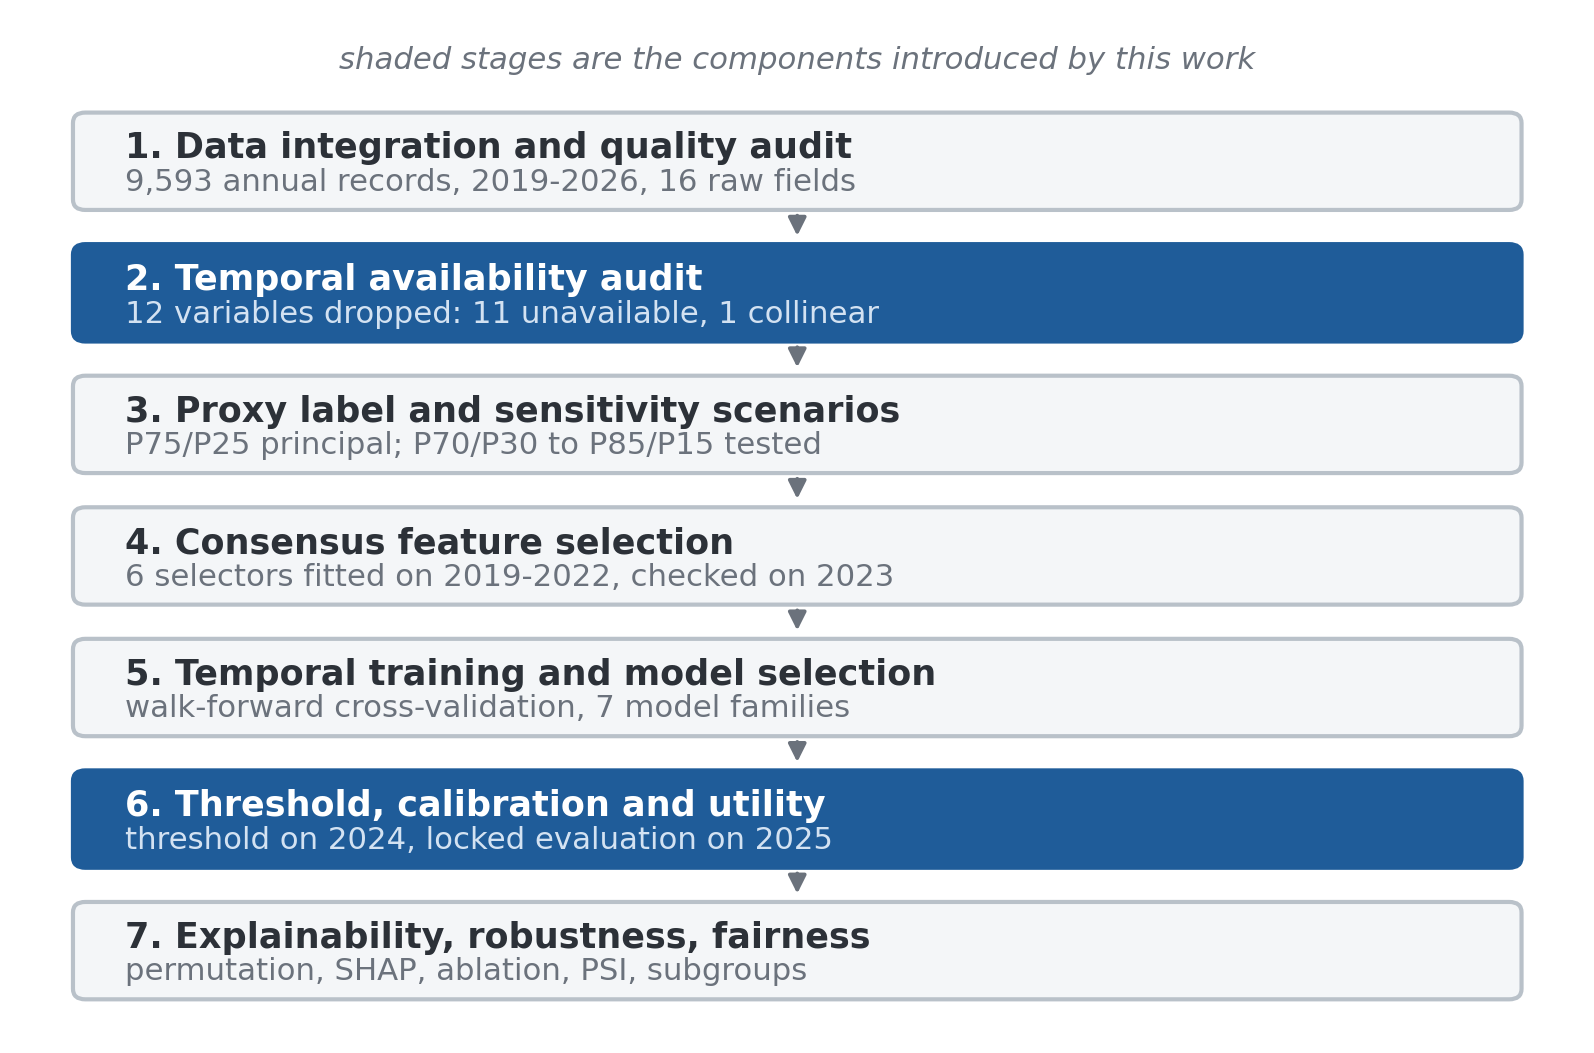
\includegraphics[width=0.86\textwidth]{figures/fig01_framework.png}
\caption[Stages of the proposed framework]{\textbf{Stages of the proposed framework.} The framework extends a conventional predictive pipeline with explicit temporal availability auditing, role-separated temporal evaluation, and joint assessment of discrimination, calibration and decision utility. The availability audit is repeated after feature selection so that the final fitted matrix, rather than only the intended exclusion rule, determines the audit outcome.}
\end{figure}

\subsection{Data source and unit of analysis}

The study uses the \emph{Casos Fiscales} data set published by the Public Prosecutor's Office of Peru (Ministerio P\'ublico -- Fiscal\'ia de la Naci\'on, MPFN) on the National Open Data Platform \cite{ministerio_publico__fiscalia_de_la_nacion_mpfn_mpfn_2022}. The registry reports, for each reporting period, the number of cases received and the number of cases processed, disaggregated by fiscal district, type of prosecution office, subject matter, specialty and case type, together with the geographic coding of the corresponding judicial district.

The unit of analysis is one \emph{operational unit-year}: the annual aggregate for a specific combination of territory, office type, subject matter, specialty and case type. The consolidated file contains 9{,}593 such records for the period 2019--2026 (Table~\ref{tab:dataset}). The 2026 file is partial, covering January to May only, and is treated throughout as exploratory.

\begin{table}[h]
\caption{Composition of the integrated data set and prevalence of the proxy label by year}\label{tab:dataset}
\begin{tabular}{lrrrrl}
\toprule
Year & Records & Cases received & Cases processed & Proxy risk (\%) & Coverage \\
\midrule
2019 & 1196 & 1400736 & 1220349 & 11.54 & Full year \\
2020 & 1142 & 863288 & 688925 & 19.44 & Full year \\
2021 & 1252 & 1298697 & 1140369 & 13.42 & Full year \\
2022 & 1272 & 1404619 & 1275920 & 12.42 & Full year \\
2023 & 1214 & 1503919 & 1376760 & 13.51 & Full year \\
2024 & 1195 & 1527838 & 1406901 & 13.31 & Full year \\
2025 & 1199 & 1492353 & 1363570 & 14.35 & Full year \\
2026 & 1123 & 622744 & 530831 & 20.21 & January--May \\
\midrule
Total & 9593 & 10114194 & 9003625 & 14.68 & \\
\bottomrule
\end{tabular}
\footnotetext{Proxy risk is the prevalence of the P75/P25 label defined in Section~\ref{sec:target}. The 2026 totals are not comparable with the preceding rows because the file covers five months.}
\end{table}

Two fields carry missing values: the specialised-unit descriptor, absent in 72.39\% of records (6{,}944 rows), which reflects that most units are not designated as specialised and is therefore encoded as an explicit category rather than imputed; and the processed-case count, absent in 0.27\% (26 rows), imputed with the training-partition median. A binary missingness indicator is retained for each affected field.

\subsection{The prediction time point and the temporal availability audit}\label{sec:availability}

The framework predicts, for a given operational unit and a given calendar year $Y$, whether that unit will exhibit the overload signal defined in Section~\ref{sec:target} once the records for $Y$ are closed. The prediction is issued \emph{at the start of $Y$}, before any of the case flow of $Y$ has been observed. Everything that follows is a consequence of that definition.

Each candidate variable was therefore assigned to one of three availability classes (Table~\ref{tab:availability}):

\begin{description}
\item[Ex ante.] Observable before year $Y$ begins. This covers the structural attributes of the operational unit --- fiscal district, department, province, judicial district, geographic code, office type, subject matter, specialty, case type and specialised designation --- their second-order interactions, the frequency encodings derived from them on the training partition, calendar indicators fixed in advance, and lagged aggregates computed strictly from years earlier than $Y$.
\item[Concurrent.] Observable only as year $Y$ unfolds. This covers cases received, cases processed and the three derived quantities that follow from them.
\item[Ex post.] Observable only once the annual file has been compiled and published: the reporting-period descriptor, the file download and cut-off dates, and the file-provenance identifier.
\end{description}

The intended predictor set contains only ex ante variables. Concurrent variables are inadmissible because they unfold during the target year and, in this study, also define the proxy outcome. Ex post variables are inadmissible because they are generated by the publication process rather than by the underlying prosecutorial operation. The distinction is enforced as a protocol criterion and then audited again after feature selection.

The second audit exposed a residual feature alignment issue. Of the fields classified as ex post, the constant file-provenance field was removed before selection, but the reporting-period descriptor, download date, cut-off date and remaining file-origin information entered the candidate pool. Three one-hot indicators derived from these fields were subsequently nominated by the consensus selector and therefore remain among the 74 features of the reported model. Each fires only for records belonging to a single training year and consequently behaves as a year-specific fixed effect. Because the three indicators are identically zero in 2024, 2025 and 2026, they cannot directly alter any reported evaluation prediction. They nevertheless violate the intended availability criterion because the fitted model was allowed to absorb year-specific information that would not be available to a deployed system.

This residual exposure is treated as a methodological finding rather than as an implementation detail. This study provides that an availability rule applied only before feature selection is insufficient: the admissibility of the final fitted matrix must be verified after all transformations and selection steps have been completed. We therefore define the post-selection matrix audit as an explicit component of the framework. Re-fitting the model on the rigorously ex ante subset remains necessary before deployment, but the present study deliberately reports the audited configuration and does not represent it as availability-audited feature.

We draw the methodological conclusion this invites, because it is the sharpest evidence in this paper for the argument the paper makes. An availability criterion that is declared in the protocol but not enforced against the feature matrix that is actually fitted does not prevent the leakage it describes. The exposure was found here only because the audit was re-run against the final list of 74 features rather than against the intended exclusion rule, and we recommend that verification --- audit the matrix, not the intention --- as an explicit step of the protocol rather than an implicit consequence of it. Re-fitting the selection and the model on the ex ante subset alone remains a prerequisite for deployment, and is listed as such in Section~\ref{sec:limits}.

\begin{table}[h]
\caption{Temporal availability audit of the candidate predictor blocks}\label{tab:availability}
\begin{tabular}{p{3.1cm}p{2.0cm}p{6.1cm}}
\toprule
Variable block & Availability & Disposition and rationale \\
\midrule
\vr Territorial and institutional attributes; their pairwise interactions; training-fitted frequency encodings & Ex ante & \textbf{Retained.} Structural properties of the operational unit, stable from one year to the next and known before the reporting year opens. \\
\vr Lagged annual aggregates and year-on-year growth rates by fiscal district & Ex ante & \textbf{Retained.} Computed exclusively from years rigorously earlier than the target year; the same-year record never enters its own history. \\
\vr Pandemic-period and post-pandemic calendar indicators & Ex ante & \textbf{Retained.} Fixed by the calendar before the year begins. \\
\vr Cases received; cases processed & Concurrent & \textbf{Excluded.} Accumulate during the target year and are unknown when the prediction is issued. \\
\vr Case balance; processing rate; balance ratio & Concurrent & \textbf{Excluded.} Derived from the concurrent block and, in addition, used to construct the label. \\
\vr Proxy-label variants for the four threshold scenarios; the principal label & Concurrent & \textbf{Excluded.} Direct functions of the outcome. \\
\vr Centred year index & Ex ante & \textbf{Excluded.} Collinear with the calendar year and extrapolates outside the training range. \\
\vr Reporting-period descriptor; download date; cut-off date; file-provenance and file-origin identifiers & Ex post & \textbf{Inadmissible; residual exposure detected after selection.} Generated when the annual file is compiled and released, and effectively encode the reporting year. Only the constant file-provenance field was dropped before selection; three indicators derived from the remaining fields survived into the reported model (Section~\ref{sec:availability}). \\
\bottomrule
\end{tabular}
\end{table}

\subsection{Proxy label construction and sensitivity}\label{sec:target}

Peru publishes no official certification of prosecutorial congestion, so the target is an auditable proxy rather than a ground truth. For each operational unit-year we define the case balance $b = R - P$ and the processing rate $r = P/R$, where $R$ and $P$ are the cases received and processed. A unit-year is labelled positive when it lies simultaneously in the upper tail of the balance distribution and the lower tail of the processing-rate distribution:
\begin{equation}
y = \mathbb{I}\big[\, b \geq q_{\alpha}(b) \;\wedge\; r \leq q_{1-\alpha'}(r) \,\big],
\end{equation}
where both quantiles are estimated \emph{on the training partition only} and then applied unchanged to every later year, so that the definition of the label is fixed before any evaluation data are seen.

Four scenarios were evaluated (Table~\ref{tab:scenarios}). The P75/P25 scenario was adopted as the principal reporting specification: It provides a moderate event prevalence and comparatively stable prevalence across the observed annual series, while the stricter scenarios represent progressively more selective overload conditions and P70/P30 is retained as an early-warning alternative.

\begin{table}[h]
\caption{Proxy label scenarios and the temporal stability of their prevalence}\label{tab:scenarios}
\begin{tabular}{lrrrrrrl}
\toprule
& \multicolumn{2}{c}{Training thresholds} & \multicolumn{4}{c}{Prevalence} & \\
\cmidrule(lr){2-3}\cmidrule(lr){4-7}
Scenario & Balance & Rate & Train & 2024 & 2025 & CV & Role \\
\midrule
P70/P30 & 7 & 0.9352 & 0.1935 & 0.1983 & 0.2002 & 0.165 & Early warning \\
\textbf{P75/P25} & \textbf{11} & \textbf{0.9162} & \textbf{0.1399} & \textbf{0.1331} & \textbf{0.1435} & \textbf{0.219} & \textbf{Principal} \\
P80/P20 & 17 & 0.8889 & 0.0927 & 0.0879 & 0.0901 & 0.278 & Severe overload \\
P85/P15 & 29 & 0.8571 & 0.0533 & 0.0544 & 0.0500 & 0.379 & Extreme cases \\
\bottomrule
\end{tabular}
\footnotetext{CV is the coefficient of variation of annual prevalence across 2019--2026. Thresholds are quantiles of the training partition (2019--2023) and are held fixed for all later years.}
\end{table}

No expert elicitation was carried out, so what follows is an internal consistency check rather than construct validation. Cliff's delta between the positive and negative classes is $-0.904$ for the case balance and $0.809$ for the processing rate. These values are large by construction, since the two quantities define the label, and we report them only to confirm that the rule was applied as specified; they are not evidence that the label measures institutional overload. The association of the label with the administrative attributes that remain admissible as predictors is by contrast weak, with Cram\'er's $V$ reaching at most 0.267 (case type) and 0.229 (office type). That asymmetry is the empirical statement of the problem the model faces: the label is defined by quantities the model is not allowed to see, and must be recovered from structural attributes that are only weakly associated with it. The only evidence bearing on the validity of the construct itself is its convergence with an unsupervised partition of the admissible predictors, reported in Section~\ref{sec:results}, and it is qualified in Section~\ref{sec:limits}.

One further property of the label follows from the missing-data treatment described above. The processed-case count is one of the two quantities that construct the label, and it is absent for 26 unit-years, which are imputed with the training-partition median. Up to 26 of the 9{,}593 labels are therefore derived in part from an imputed value rather than from a reported one. The proportion is small, and a missingness indicator is retained, but the labels concerned are not observations in the same sense as the rest and we note the fact here rather than only in the description of the data.

\subsection{Feature engineering}

Fourteen derived variables were constructed in four families: operational pressure indicators; calendar descriptors; second-order categorical interactions (subject matter $\times$ office type, judicial district $\times$ case type, office type $\times$ specialty); and lagged historical aggregates by fiscal district. The historical family deserves a specific note, because it is the most common source of subtle leakage in panel data of this kind. Each lagged feature is computed as an expanding mean over the \emph{previous} years of the same fiscal district, obtained by shifting the annual series one period before aggregation; missing values at the start of each series are filled with the training-partition median. No record therefore contributes to its own history.

High-cardinality categorical variables were frequency-encoded with frequencies estimated on the training partition alone and mapped onto later partitions, with unseen categories assigned zero. Remaining categorical variables were one-hot encoded. Numerical variables were median-imputed and standardised. All encoders, imputers and scalers were fitted exclusively on the training partition, giving 564 preprocessed candidate features.

\subsection{Consensus feature selection}\label{sec:selection}

Six complementary selectors were applied: mutual information, ANOVA $F$-test and $\chi^2$ (filters); Random Forest importance (embedded); and Boruta \cite{kursa_feature_2010} and recursive feature elimination with cross-validation (wrappers). Each selector nominated its top 40 features, and a stability score was computed as the proportion of selectors nominating each feature. Features receiving at least two of six votes were retained, giving a final set of 74. The purpose of the consensus step is not to identify a universally optimal subset, but to reduce dependence on the inductive bias of any single selector while preserving a transparent rule for inclusion. Because selection can itself introduce temporal exposure if fitted outside the training window, its fitting and verification are explicitly constrained by the partition protocol.

The selection stage was confined to the earliest part of the training block: selectors and their preprocessing were fitted on 2019--2022 and the resulting subset was checked on 2023, a year that is still internal to the training partition and therefore never used for reporting. That internal check gave an F1-score of 0.456, a ROC-AUC of 0.800 and a balanced accuracy of 0.751, indicating that the dimensional reduction from 564 to 74 features did not degrade the signal.

\subsection{Partition protocol}\label{sec:protocol}

Each temporal partition has a pre-specified role and an explicitly delimited set of permitted operations:

\begin{enumerate}
\item \textbf{Feature selection} --- 2019--2022, with an internal check on 2023. Never used for reporting.
\item \textbf{Model training and hyperparameter search} --- 2019--2023 ($n = 6{,}076$), using year-block walk-forward cross-validation internal to this block, so that every inner fold trains on earlier years and validates on a later one.
\item \textbf{Decision-threshold selection and conformal calibration} --- 2024 ($n = 1{,}195$). This is the only data set consulted when choosing the operating point, and it is used for no other purpose.
\item \textbf{Locked evaluation} --- 2025 ($n = 1{,}199$). Consulted once, after the model and threshold were frozen. Every headline figure in Section~\ref{sec:results} refers to this partition.
\item \textbf{Exploratory temporal check} --- 2026 ($n = 1{,}123$), a five-month file reported separately and never used to support a performance claim.
\end{enumerate}

Because the threshold is selected on 2024 and the evaluation is performed on 2025, no quantity reported as a final result was optimised on the data that produced it.

\begin{figure}[h]
\centering
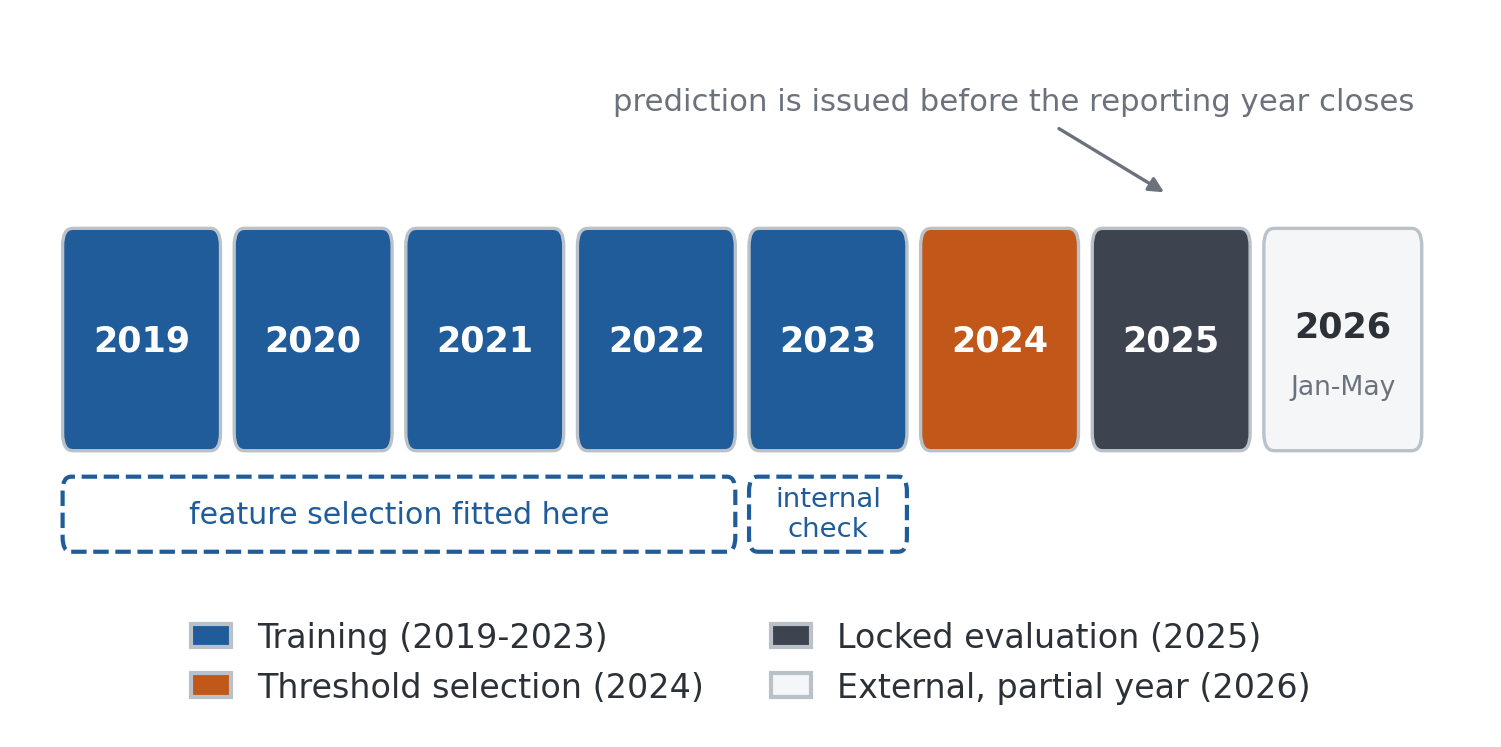
\includegraphics[width=0.94\textwidth]{figures/fig02_protocol.png}
\caption[Temporal partition protocol]{\textbf{Temporal partition protocol.} Feature selection is confined to 2019--2022 with an internal check on 2023; the decision threshold is chosen on 2024; 2025 serves as the single locked evaluation set; the partial 2026 file is exploratory only.}\label{fig:protocol}
\end{figure}

\begin{table}[h]
\caption{Role, size and label prevalence of each partition}\label{tab:partitions}
\begin{tabular}{llrrp{4.4cm}}
\toprule
Partition & Years & Records & Prevalence (\%) & Role \\
\midrule
Training & 2019--2023 & 6076 & 13.99 & Fitting all preprocessors, selectors and models; internal walk-forward CV \\
Validation & 2024 & 1195 & 13.31 & Decision-threshold selection and conformal calibration only \\
Test & 2025 & 1199 & 14.35 & Single locked evaluation \\
Temporal check & 2026 & 1123 & 20.21 & Exploratory temporal generalisation; partial year \\
\bottomrule
\end{tabular}
\end{table}

\subsection{Models, hyperparameter search and evaluation}

Seven model families were trained on the 74 selected features: a majority-class baseline, $\ell_1$/$\ell_2$-regularised logistic regression, a calibrated linear support vector machine, XGBoost \cite{chen_xgboost_2016}, LightGBM \cite{ke_lightgbm_2017}, CatBoost \cite{prokhorenkova_catboost_2018}, and a LightGBM variant tuned with Optuna \cite{akiba_optuna_2019}. Soft-voting and temporally stacked ensembles were also evaluated. Class imbalance was handled by cost-sensitive weighting rather than synthetic resampling. Hyperparameters were searched by randomised search under the same year-block walk-forward scheme used for training. All modelling used scikit-learn \cite{pedregosa_scikitlearn_2011}. The training partition contains 850 positive unit-years against the 74 selected features, an events-per-variable ratio of approximately 11.5. Every stochastic component of the pipeline --- the randomised search, the bootstrap, the permutation importance, the clustering and the shadow features of the Boruta selector --- was seeded from a single fixed random state (42).

Two additional benchmarks frame the results. \emph{Single-indicator rules} threshold the case balance or the processing rate directly at their training quantiles; they are reported because they establish what could be achieved by a decision maker who already knows the outcome year's volumes. An \emph{oracle check} reproduces the conjunction that defines the label; it attains perfect scores by construction and is reported only as a sanity check, never as a comparator.

Evaluation reports discrimination (ROC-AUC, PR-AUC), threshold-dependent operating characteristics (precision, recall, F1, specificity, Matthews correlation coefficient), calibration (Brier score \cite{brier_verification_1950}, expected and maximum calibration error, reliability bins with signed deviations), and decision-analytic utility. Uncertainty is quantified by bootstrap resampling of the evaluation partition with 300 iterations, with intervals taken as the 2.5th and 97.5th percentiles of the resampled distribution. The 300-resample bootstrap provides indicative rather than high-precision uncertainty intervals. These intervals are retained as descriptive uncertainty estimates, and the number of resamples should be increased in a future confirmatory analysis.
For decision-analytic utility we compute the net benefit \cite{vickers_decision_2006}
\begin{equation}\label{eq:nb}
\mathrm{NB}(p_t) = \frac{\mathrm{TP}(p_t)}{n} - \frac{\mathrm{FP}(p_t)}{n}\cdot\frac{p_t}{1-p_t},
\end{equation}
where $p_t$ is the threshold probability at which a decision maker would be indifferent between acting and not acting, and compare it against the two reference policies of flagging every unit ($\mathrm{NB} = \pi - (1-\pi)\,p_t/(1-p_t)$ for prevalence $\pi$) and flagging none ($\mathrm{NB} = 0$).

Population stability indices, an ablation study over feature blocks, a stress test under perturbation of the operational attributes, subgroup performance analysis \cite{hardt_equality_2016} and split-conformal prediction \cite{vovk_algorithmic_2005,angelopoulos_conformal_2023} complete the assessment. The full software stack is listed in Table~\ref{tab:software}.

\begin{table}[h]
\caption{Software environment}\label{tab:software}
\begin{tabular}{llllll}
\toprule
Component & Version & Component & Version & Component & Version \\
\midrule
Python & 3.12.13 & scikit-learn & 1.6.1 & CatBoost & 1.2.10 \\
pandas & 2.2.2 & LightGBM & 4.6.0 & SHAP & 0.52.0 \\
NumPy & 2.0.2 & XGBoost & 3.3.0 & Optuna & 4.9.0 \\
\bottomrule
\end{tabular}
\end{table}

\subsection{Reporting standard and use of generative AI}

The study is reported in accordance with the TRIPOD+AI statement for the reporting of prediction model studies that use machine learning \cite{collins_tripod_2024}; the completed checklist is provided as Additional file~1. Where TRIPOD+AI asks for a single summary of performance we depart from it deliberately, reporting discrimination, calibration and decision-analytic utility separately for the reasons set out in Section~\ref{sec:intro}.

% TODO(authors): confirm this disclosure is accurate before submission, and amend it if not.
Generative artificial intelligence and large language models were not used to design the study, to generate or analyse the data, or to derive any result reported in this article. Their use was confined to language editing of the manuscript text; the authors reviewed all such edits and take full responsibility for the content of the article.

\section{Results}\label{sec:results}

\subsection{Temporal behaviour of the workload and the label}

Figure~\ref{fig:temporal} shows the annual volumes and the prevalence of the proxy label. Case flow contracted sharply in 2020 --- received cases fell by 38\% relative to 2019 --- and recovered to above pre-pandemic levels by 2022. Label prevalence tracks that disruption, peaking at 19.44\% in 2020, settling in a narrow band of 12.4--14.4\% from 2021 to 2025, and rising to 20.21\% in the partial 2026 file. The 2026 figure should not be read as a trend: a five-month window truncates the processing of cases received late in the window and mechanically inflates the measured balance.

\begin{figure}[h]
\centering
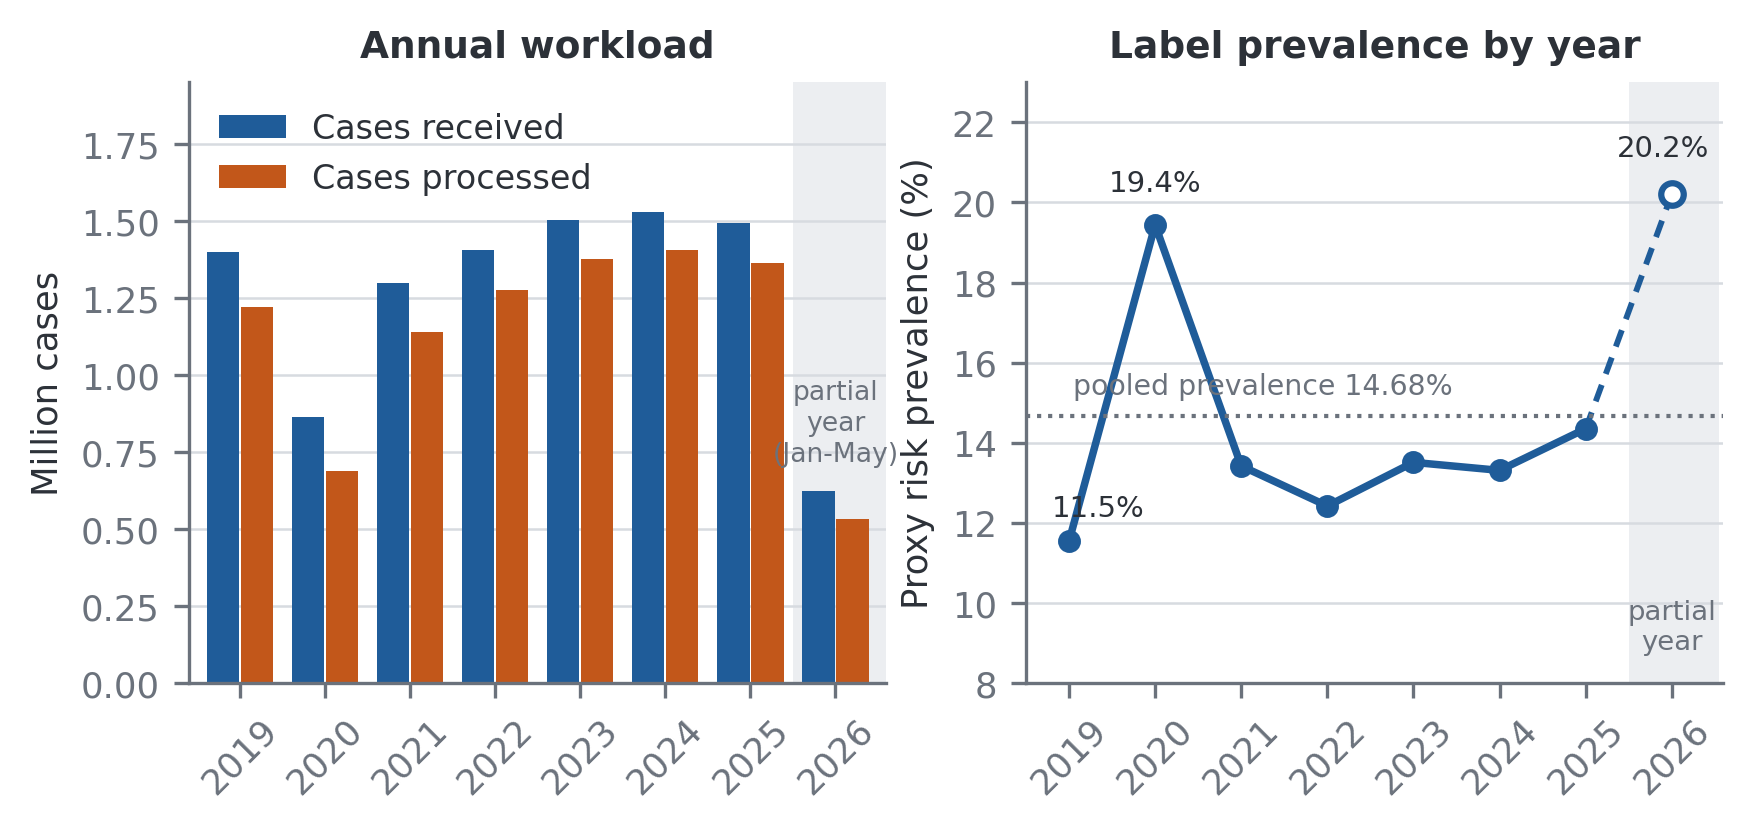
\includegraphics[width=0.98\textwidth]{figures/fig03_temporal.png}
\caption[Annual case volumes and proxy label prevalence, 2019--2026]{\textbf{Annual case volumes and proxy label prevalence, 2019--2026.} Left: cases received and cases processed by year. Right: prevalence of the proxy overload label. The 2026 file covers January to May only, so its volumes are not comparable with the preceding years and its prevalence is inflated by truncation; it is shaded in both panels, and the segment leading to it is dashed with a hollow marker rather than joined as a trend.}\label{fig:temporal}
\end{figure}

\subsection{Model comparison}

Table~\ref{tab:models} reports the seven model families on the locked 2025 evaluation at the reference threshold of 0.50, alongside the two ensembles and the two benchmark classes. The learned models form a clear boosting-dominated performance group, but the results do not support a unique winner within that family. The differences between CatBoost and each of the other three boosting configurations are statistically significant but numerically small (DeLong $p = 0.0026$--$0.0038$; absolute AUC differences of 0.023--0.036). Applying Holm's step-down correction across the four DeLong comparisons reported here raises all three of those $p$-values to 0.0104, which leaves the conclusion unchanged; we report the corrected values because the comparisons are made on the locked partition and multiplicity is otherwise unaccounted for. The Friedman test across four temporal folds rejects the hypothesis of equal F1 across the five base learners ($\chi^2 = 11.4$, $p = 0.022$), but the Nemenyi post-hoc comparison identifies no significant pair at the 5\% level, the smallest adjusted $p$-value being 0.056 for the support vector machine against LightGBM and CatBoost. We therefore report the boosting family as a performance plateau rather than claiming a single winner.

XGBoost was fixed as the reported reference configuration before the 2025 partition was opened, on the basis of walk-forward cross-validated F1 computed strictly inside the training block. The cross-validated differences among XGBoost, CatBoost and LightGBM were smaller than the corresponding fold-to-fold variability, so the choice should not be interpreted as evidence that XGBoost is comparatively higher performance under the specified selection criterion. We retain XGBoost as the reference configuration for consistency with the pre-specified reporting pipeline.

\begin{table}[h]
\caption{Performance on the locked 2025 evaluation set at the reference threshold of 0.50}\label{tab:models}
\begin{tabular}{lrrrrrr}
\toprule
Model & Precision & Recall & F1 & ROC-AUC & PR-AUC & MCC \\
\midrule
\multicolumn{7}{l}{\emph{Learned models (reported configuration)}}\\
Majority-class baseline & 0.000 & 0.000 & 0.000 & 0.500 & 0.143 & 0.000 \\
Logistic regression & 0.326 & 0.645 & 0.433 & 0.783 & 0.359 & 0.327 \\
Support vector machine & 0.457 & 0.122 & 0.193 & 0.791 & 0.370 & 0.178 \\
XGBoost & 0.522 & 0.407 & 0.458 & 0.796 & 0.400 & 0.383 \\
LightGBM & 0.455 & 0.471 & 0.463 & 0.793 & 0.502 & 0.371 \\
CatBoost & 0.449 & 0.541 & 0.491 & \textbf{0.819} & 0.457 & 0.399 \\
Soft-voting ensemble & 0.488 & 0.465 & 0.476 & 0.817 & 0.502 & 0.391 \\
Temporal stacking ensemble & 0.368 & 0.640 & 0.467 & 0.817 & 0.506 & 0.369 \\
\midrule
\multicolumn{7}{l}{\emph{Reference benchmarks (use concurrent information; not deployable)}}\\
Balance-only rule & 0.513 & 1.000 & 0.679 & 0.945 & 0.658 & 0.657 \\
Processing-rate-only rule & 0.548 & 1.000 & 0.708 & 0.914 & 0.452 & 0.687 \\
Label-definition oracle & 1.000 & 1.000 & 1.000 & 1.000 & 1.000 & 1.000 \\
\bottomrule
\end{tabular}
\footnotetext{The reference benchmarks are computed from the concurrent variables that the availability audit excludes from the learned models; they are reported to bound the problem, not as competitors. The oracle reproduces the rule that defines the label and is a sanity check only.}
\end{table}

The benchmark block is the most informative row group in the table, and it is the reason the temporal evaluation protocol is presented with the caveats that follow. The two single-indicator rules outperform every learned model by a wide margin --- an F1 of 0.708 for the processing-rate rule against 0.458 for XGBoost. This is not evidence that the machine learning pipeline is poorly constructed. It is a direct measurement of how much of the label is carried by information that does not exist at the prediction time point. The rules read the outcome year's volumes; the models are forbidden from doing so. The gap between the two is the price of a genuinely ex ante prediction, and any study that reports rule-level performance from a model trained on concurrent variables is measuring the label's own definition rather than a forecast.

\subsection{Temporal robustness}

Walk-forward validation (Figure~\ref{fig:walkforward}) trains on all years up to $t-1$ and evaluates on year $t$. Across the six folds that evaluate a complete year --- 2020 through 2025 --- ROC-AUC stays within 0.834--0.895 with no downward trend, and F1 within 0.542--0.581. A seventh fold evaluates the partial 2026 file (ROC-AUC 0.894, F1 0.664) and is plotted for completeness only; consistent with the protocol of Section~\ref{sec:protocol} it supports no claim made in this paper, and the ranges quoted above exclude it.

These fold-level figures are not comparable with the locked evaluation, and the gap is worth stating explicitly because Figure~\ref{fig:walkforward} and Table~\ref{tab:final} both report on 2025. The walk-forward fold for 2025 attains a ROC-AUC of 0.851; the frozen model of Table~\ref{tab:final} attains 0.796 on the same year. The two differ in their training window --- 2019--2024 for the fold against 2019--2023 for the frozen model --- and each fold also refits its preprocessing on its own window, so the comparison is indicative rather than a controlled contrast. It nonetheless bounds the order of magnitude of what the recency of the training window contributes, and it is the reason the walk-forward curve should not be read as an estimate of deployed performance.

Nested temporal cross-validation over four outer folds gives an out-of-fold F1 of $0.549 \pm 0.048$ for LightGBM, $0.531 \pm 0.032$ for CatBoost and $0.454 \pm 0.040$ for logistic regression. This reproduces the separation between the boosting family and logistic regression seen in Table~\ref{tab:models}, but not the ordering inside that family: LightGBM and CatBoost exchange places between the two criteria, and under both the fold-to-fold variability exceeds the between-model differences.

\begin{figure}[h]
\centering
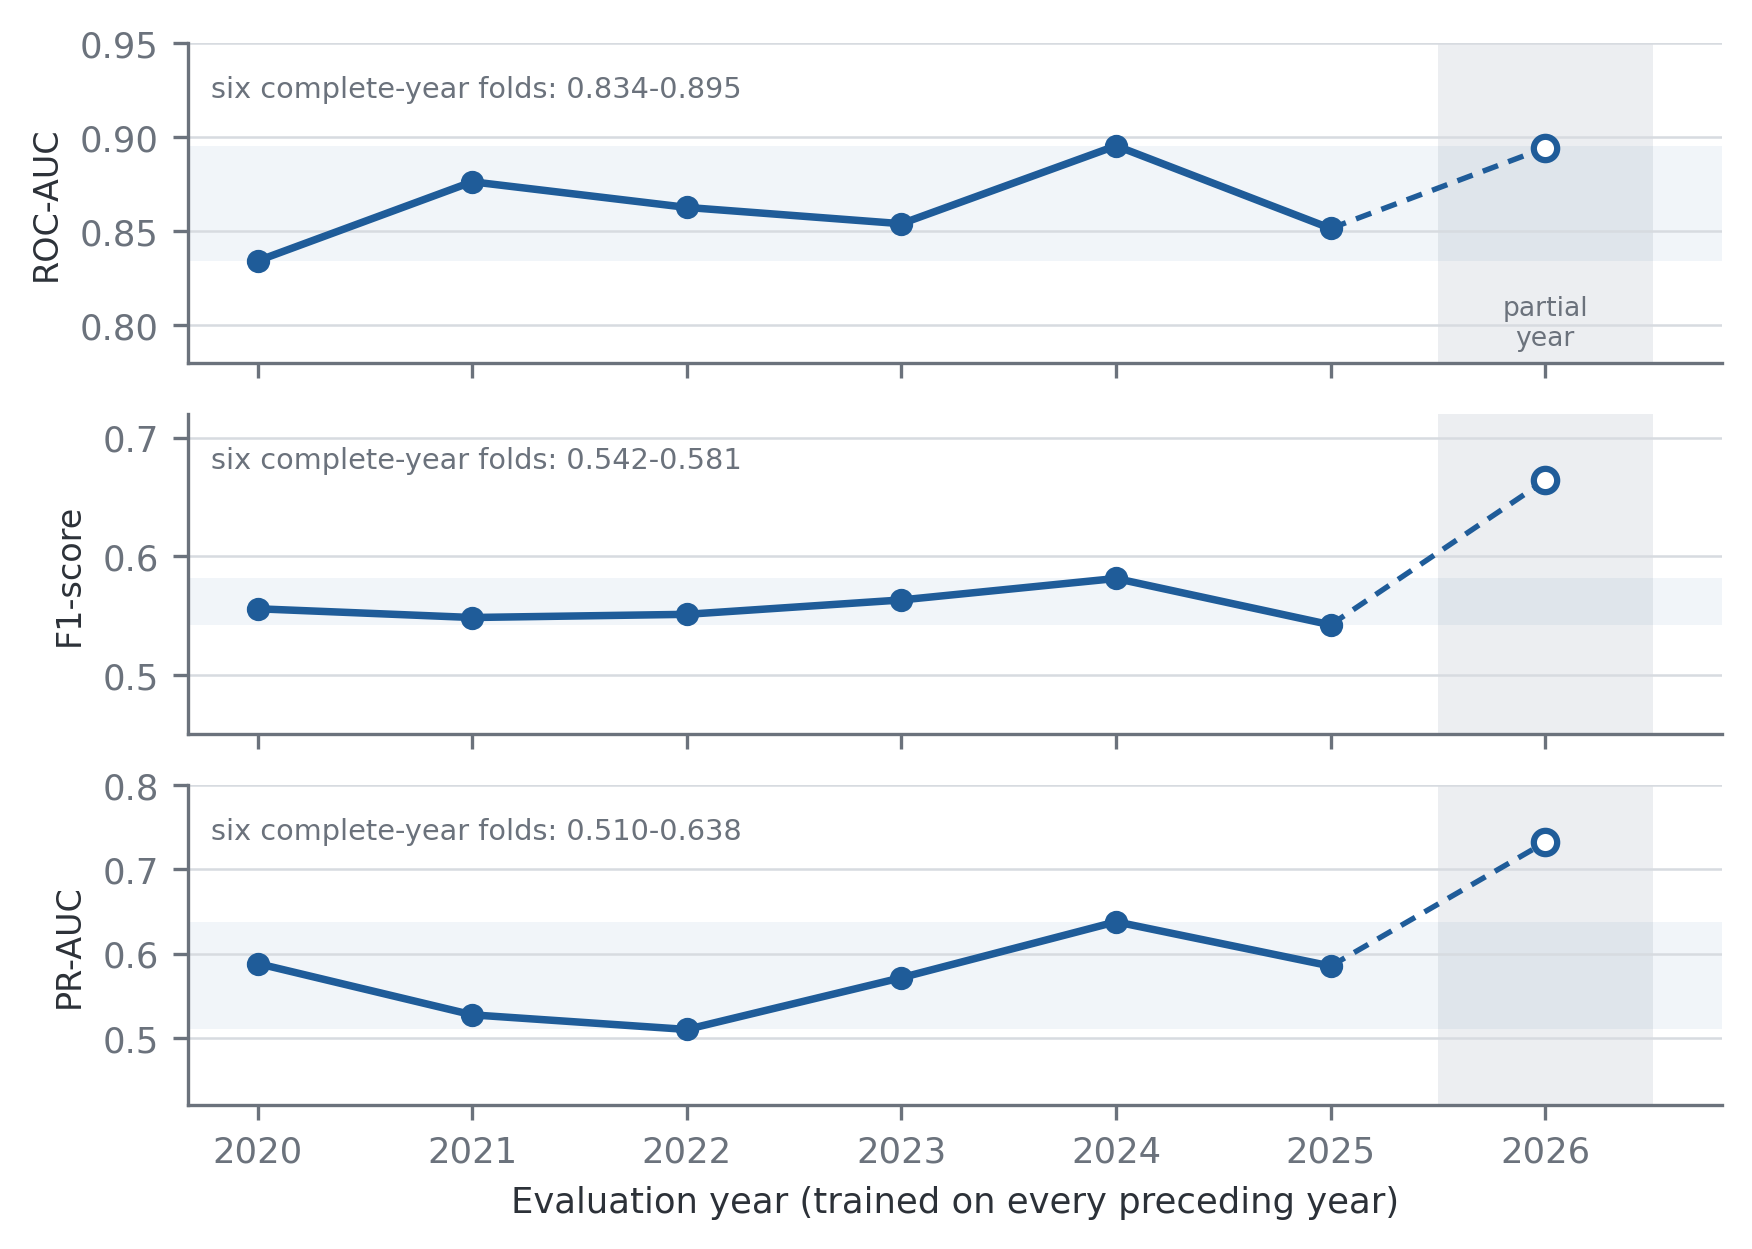
\includegraphics[width=0.80\textwidth]{figures/fig04_walkforward.png}
\caption[Walk-forward validation across annual folds]{\textbf{Walk-forward validation across annual folds.} Each point trains on every preceding year and evaluates on the year shown; one panel per metric, so each is read on the scale that makes its own variation legible. The shaded horizontal band and the annotation give the range over the six folds that evaluate a complete year (2020--2025). The 2026 fold evaluates a five-month file: it is separated by a wash, drawn with a hollow marker and a dashed connector, and excluded from every range quoted here and in the text.}\label{fig:walkforward}
\end{figure}

The learning curve (Figure~\ref{fig:learning}) shows training F1 declining from 0.948 to 0.900 as the sample grows while cross-validated F1 rises from 0.217 to 0.490 and then flattens. The gap of 0.41 at the largest training size does not close, which indicates that the ceiling is set by the weak association between the admissible predictors and the label, not by the volume of data. Adding more years of the same registry would not be expected to change this.

\begin{figure}[h]
\centering
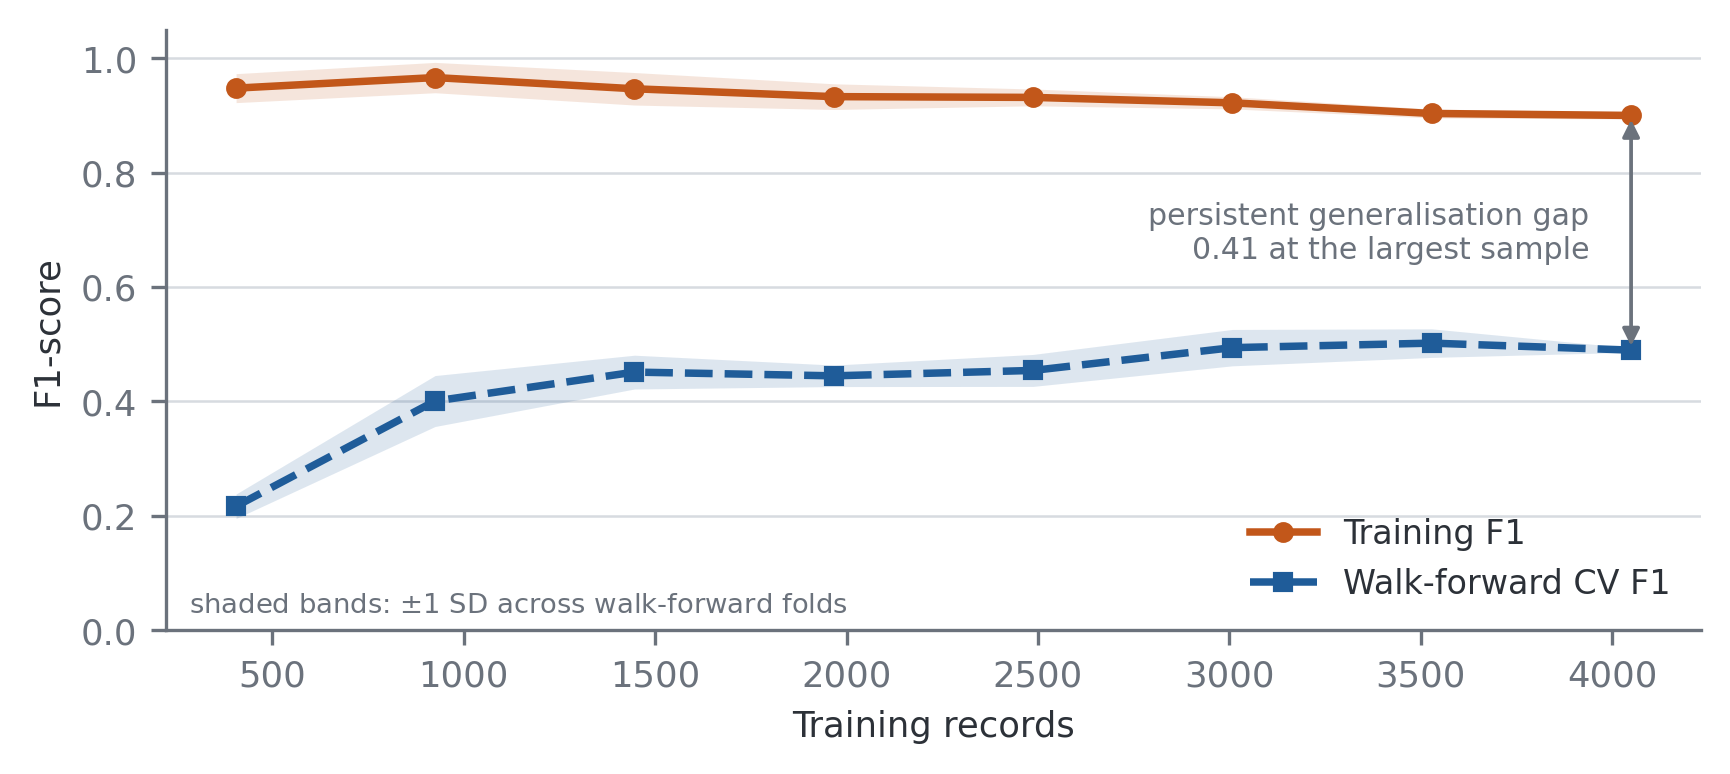
\includegraphics[width=0.90\textwidth]{figures/fig05_learning_curve.png}
\caption[Learning curve for the reported configuration]{\textbf{Learning curve for the reported configuration.} The persistent gap between training and walk-forward cross-validated F1 reflects the limited signal available in ex ante predictors, not an insufficient sample.}\label{fig:learning}
\end{figure}

Population stability indices computed against the training distribution show no relevant drift for 2024 and 2025 (all PSI $< 0.03$). For the partial 2026 file, two of the five monitored quantities exceed the moderate-drift threshold (processing rate, PSI $= 0.129$; balance ratio, PSI $= 0.138$), consistent with the truncation artefact already noted. Under a stress test that perturbs the operational attributes, F1 degrades from 0.409 to 0.279 at a 10\% perturbation and to 0.208 at 30\%, while ROC-AUC falls only from 0.796 to 0.726, indicating that the ranking produced by the model is considerably more robust than any fixed-threshold decision derived from it --- a finding that anticipates the calibration and utility results below.

\subsection{Threshold selection and the final operating point}

Table~\ref{tab:thresholds} lists the operating points obtainable on the 2024 validation partition under four criteria. The F1-optimal threshold is $\tau = 0.65$; Youden's $J$ statistic is maximised at 0.115, a far more permissive cut; a precision of at least 0.80 requires 0.95; and a recall of at least 0.80 points to the need for 0.20. The spread of these values across almost the whole unit interval is itself a result: the choice of operating point dominates every threshold-dependent metric, and reporting a single F1 without stating how its threshold was chosen conveys very little.

\begin{table}[h]
\caption{Decision thresholds under four criteria, all selected on the 2024 validation partition}\label{tab:thresholds}
\begin{tabular}{llp{7.2cm}}
\toprule
Criterion & Threshold & Interpretation \\
\midrule
Fixed reference & 0.500 & Conventional default; rarely optimal under class imbalance \\
F1-optimal & \textbf{0.650} & Maximises F1 on 2024; adopted as the reported operating point \\
Youden's $J$ & 0.115 & Maximises sensitivity $+$ specificity $-1$ ($J = 0.662$) \\
Precision $\geq 0.80$ & 0.950 & Lowest threshold reaching the precision target \\
Recall $\geq 0.80$ & 0.200 & Highest threshold still reaching the recall target \\
\bottomrule
\end{tabular}
\end{table}

Table~\ref{tab:final} reports the frozen model at $\tau = 0.65$ across the three partitions. On the locked 2025 evaluation the model attains a ROC-AUC of 0.796 (95\% CI 0.760--0.838), a PR-AUC of 0.400 (0.330--0.480) and an F1-score of 0.409 (0.331--0.487), from 58 true positives, 54 false positives, 114 false negatives and 973 true negatives. Performance on 2024 is markedly better than on 2025 (F1 of 0.614 against 0.409), which is expected and is precisely why the threshold-selection partition cannot be used to report performance: the operating point was fitted to that partition's score distribution.

\begin{table}[h]
\caption{Frozen XGBoost model at the F1-optimal threshold $\tau = 0.65$}\label{tab:final}
\begin{tabular}{lrrrrrrr}
\toprule
Partition & Accuracy & Precision & Recall & F1 & ROC-AUC & PR-AUC & MCC \\
\midrule
Validation 2024 & 0.901 & 0.639 & 0.591 & 0.614 & 0.896 & 0.623 & 0.558 \\
\textbf{Test 2025} & \textbf{0.860} & \textbf{0.518} & \textbf{0.337} & \textbf{0.409} & \textbf{0.796} & \textbf{0.400} & \textbf{0.343} \\
Temporal check 2026 & 0.820 & 0.593 & 0.352 & 0.442 & 0.841 & 0.598 & 0.359 \\
\midrule
\multicolumn{8}{l}{\emph{Bootstrap 95\% confidence intervals, test 2025 (300 resamples)}}\\
F1 & \multicolumn{7}{l}{0.409 (0.331--0.487)} \\
ROC-AUC & \multicolumn{7}{l}{0.796 (0.760--0.838)} \\
PR-AUC & \multicolumn{7}{l}{0.400 (0.330--0.480)} \\
\bottomrule
\end{tabular}
\footnotetext{The 2024 row is reported for completeness only. Because the threshold was selected on that partition, its metrics are optimistically biased and are not comparable with the 2025 row. The 2026 row refers to a five-month file.}
\end{table}

\subsection{Calibration: magnitude and direction of the deviation}\label{sec:calibration}

The model attains a Brier score of 0.116, an expected calibration error of 0.089 and a maximum calibration error of 0.461 on the 2025 evaluation. The aggregate figures, however, conceal a systematic pattern that only the signed deviations reveal (Table~\ref{tab:calibration} and Figure~\ref{fig:calibration}).

\begin{table}[h]
\caption{Reliability bins on the 2025 evaluation set, with signed deviations}\label{tab:calibration}
\begin{tabular}{lrrrrl}
\toprule
Predicted band & $n$ & Mean pred. & Observed & Deviation & Direction \\
\midrule
0.0--0.1 & 932 & 0.011 & 0.072 & $-0.061$ & Under-estimation \\
0.1--0.2 & 64 & 0.144 & 0.234 & $-0.090$ & Under-estimation \\
0.2--0.3 & 32 & 0.248 & 0.219 & $+0.030$ & Over-estimation \\
0.3--0.4 & 16 & 0.341 & 0.375 & $-0.034$ & Under-estimation \\
0.4--0.5 & 21 & 0.450 & 0.333 & $+0.117$ & Over-estimation \\
0.5--0.6 & 17 & 0.555 & 0.529 & $+0.025$ & Over-estimation \\
0.6--0.7 & 18 & 0.663 & 0.444 & $+0.218$ & Over-estimation \\
0.7--0.8 & 10 & 0.761 & 0.300 & $\mathbf{+0.461}$ & Over-estimation \\
0.8--0.9 & 34 & 0.854 & 0.618 & $+0.236$ & Over-estimation \\
0.9--1.0 & 55 & 0.949 & 0.527 & $+0.422$ & Over-estimation \\
\bottomrule
\end{tabular}
\footnotetext{Deviation is the mean predicted probability minus the observed rate, so a positive value denotes over-estimation. Brier score 0.116; expected calibration error 0.089; maximum calibration error 0.461, attained in the 0.7--0.8 band, which holds 10 units and 3 events and therefore estimates that deviation only weakly.}
\end{table}

\begin{figure}[h]
\centering
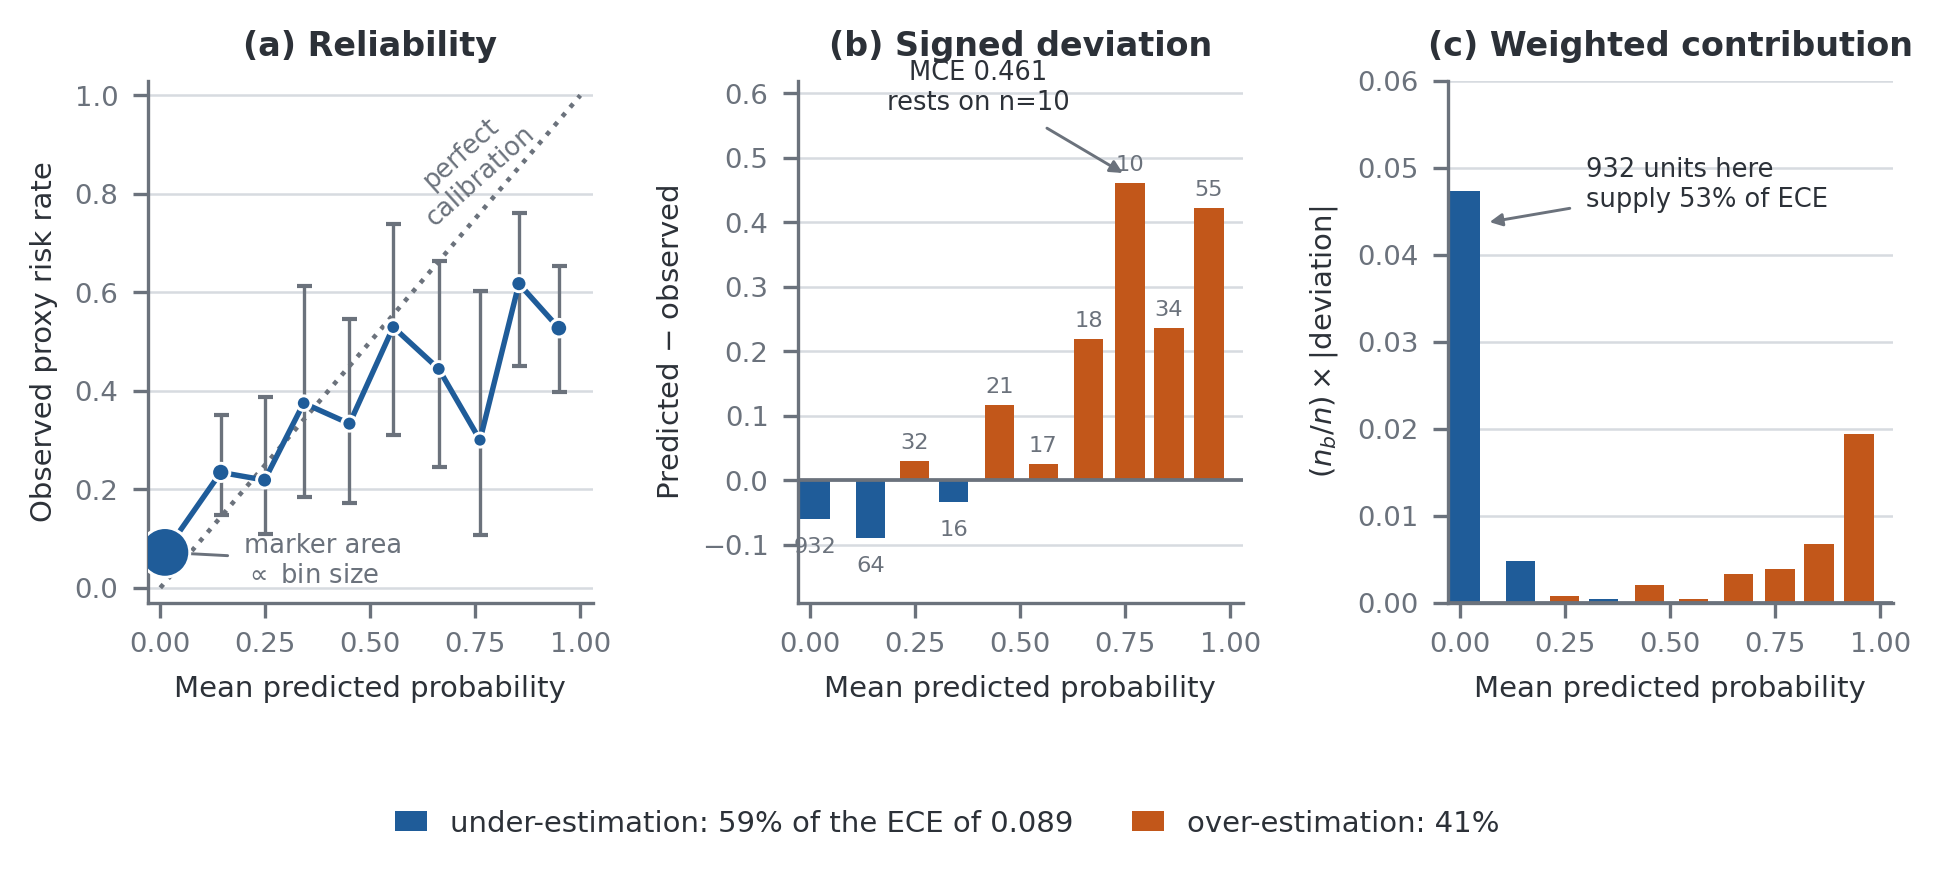
\includegraphics[width=0.98\textwidth]{figures/fig06_calibration.png}
\caption[Calibration on the 2025 evaluation set]{\textbf{Calibration on the 2025 evaluation set.} (a) Observed rate against mean predicted probability, with Wilson 95\% intervals; marker area is proportional to the number of units in the bin. (b) Signed deviation by band, each bar labelled with its bin size. (c) The same deviations weighted by bin size, which is what the expected calibration error of 0.089 sums. Above a predicted probability of 0.3 the model over-estimates risk, severely so in the highest bands; below 0.2 it under-estimates it. Panel (c) is included because panel (b) alone would misreport the result: the tallest bar rests on ten units, while the bin holding 932 of the 1{,}199 units supplies 53\% of the total error.}\label{fig:calibration}
\end{figure}

The deviation is directional. In the two lowest bands the model \emph{under-estimates} risk: units assigned a mean probability of 0.011 exhibit an observed rate of 0.072. In every band above 0.3 --- with the single exception of the sparsely populated 0.3--0.4 band --- the model \emph{over-estimates} risk, and the over-estimation grows with confidence. Units to which the model assigns a mean probability of 0.949 exhibit an observed rate of 0.527, and the maximum calibration error of 0.461 occurs in the 0.7--0.8 band, where a mean predicted probability of 0.761 corresponds to an observed rate of 0.300.

The two directions do not contribute equally to the aggregate, and the aggregate alone would misdescribe them. Decomposing the expected calibration error over the bins of Table~\ref{tab:calibration} gives 0.053 from the three under-estimating bands and 0.036 from the seven over-estimating ones, so 59\% of the total error is under-estimation --- almost all of it contributed by the 0.0--0.1 band alone, which holds 932 of the 1{,}199 units. The over-estimation above 0.3 is the operationally consequential half, because that is the region in which a decision would be taken, but it is not the larger half.

The maximum calibration error warrants a further caution. Its value of 0.461 is attained in the 0.7--0.8 band, which contains 10 units and 3 events; an exact binomial interval for that observed rate spans roughly 0.07 to 0.65, so the statistic is a moderate to low estimate. The same conclusion is supported far more robustly by the 0.9--1.0 band, where 55 units with a mean predicted probability of 0.949 exhibit an observed rate of 0.527, a signed deviation of 0.422. We report the maximum calibration error because it is a standard reporting quantity, and we report the bin size alongside it for the same reason.

This direction matters for interpretation, and it has a plausible cause. The model was trained with cost-sensitive class weighting, which raises predicted probabilities for the minority class relative to an unweighted fit, and the pattern observed here --- inflation growing with confidence --- is consistent with that mechanism. These results provide supporting alignment rather than conclusive within this scope evidence, establishing the mechanism would require refitting the same model without class weighting and comparing the reliability curves, which we did not do. The operational consequence is that a raw predicted probability from this model must not be read as an expected frequency of overload. It ranks units correctly --- the observed rate rises monotonically across the coarse strata of Section~\ref{sec:strata} --- but its absolute scale is not trustworthy. Any deployment must therefore recalibrate the scores, and the recalibration must be fitted on a data set held apart from the final evaluation; the 2024 partition, which already serves as the threshold-selection set, is the natural candidate, with the caveat that using one partition for both purposes leaves the interaction between them unmeasured. We report this as an outstanding requirement rather than a completed step: the results in this paper are those of the uncalibrated model, and we do not claim recalibrated performance we have not measured.

\subsection{Risk stratification}\label{sec:strata}

Grouping the predicted probabilities (Table~\ref{tab:strata} and Figure~\ref{fig:strata}) shows that the ranking induced by the model is sound even though its probability scale is not. The observed overload rate rises monotonically from 7.2\% in the lowest band to 52.1\% in the highest, against a base rate of 14.35\%. The two upper bands together contain 14.3\% of the operational units and 48.3\% of the overload events, while the lowest band contains 77.7\% of the units at approximately half the base rate.

\begin{table}[h]
\caption{Descriptive score strata on the 2025 evaluation set}\label{tab:strata}
\begin{tabular}{lrrrrrr}
\toprule
Stratum & Band & $n$ & Events & Observed rate & Share of units & Share of events \\
\midrule
Low & $<0.10$ & 932 & 67 & 0.072 & 77.7\% & 39.0\% \\
Moderate & 0.10--0.30 & 96 & 22 & 0.229 & 8.0\% & 12.8\% \\
High & 0.30--0.60 & 54 & 22 & 0.407 & 4.5\% & 12.8\% \\
Very high & $\geq 0.60$ & 117 & 61 & 0.521 & 9.8\% & 35.5\% \\
\midrule
All & & 1199 & 172 & 0.144 & 100\% & 100\% \\
\bottomrule
\end{tabular}
\footnotetext{Bands are fixed cut-offs of the predicted probability at 0.10, 0.30 and 0.60. Because the boundaries are defined on the uncalibrated probability scale, they are not transferable to a recalibrated model and would require re-derivation and independent validation before use.}
\end{table}

\begin{figure}[h]
\centering
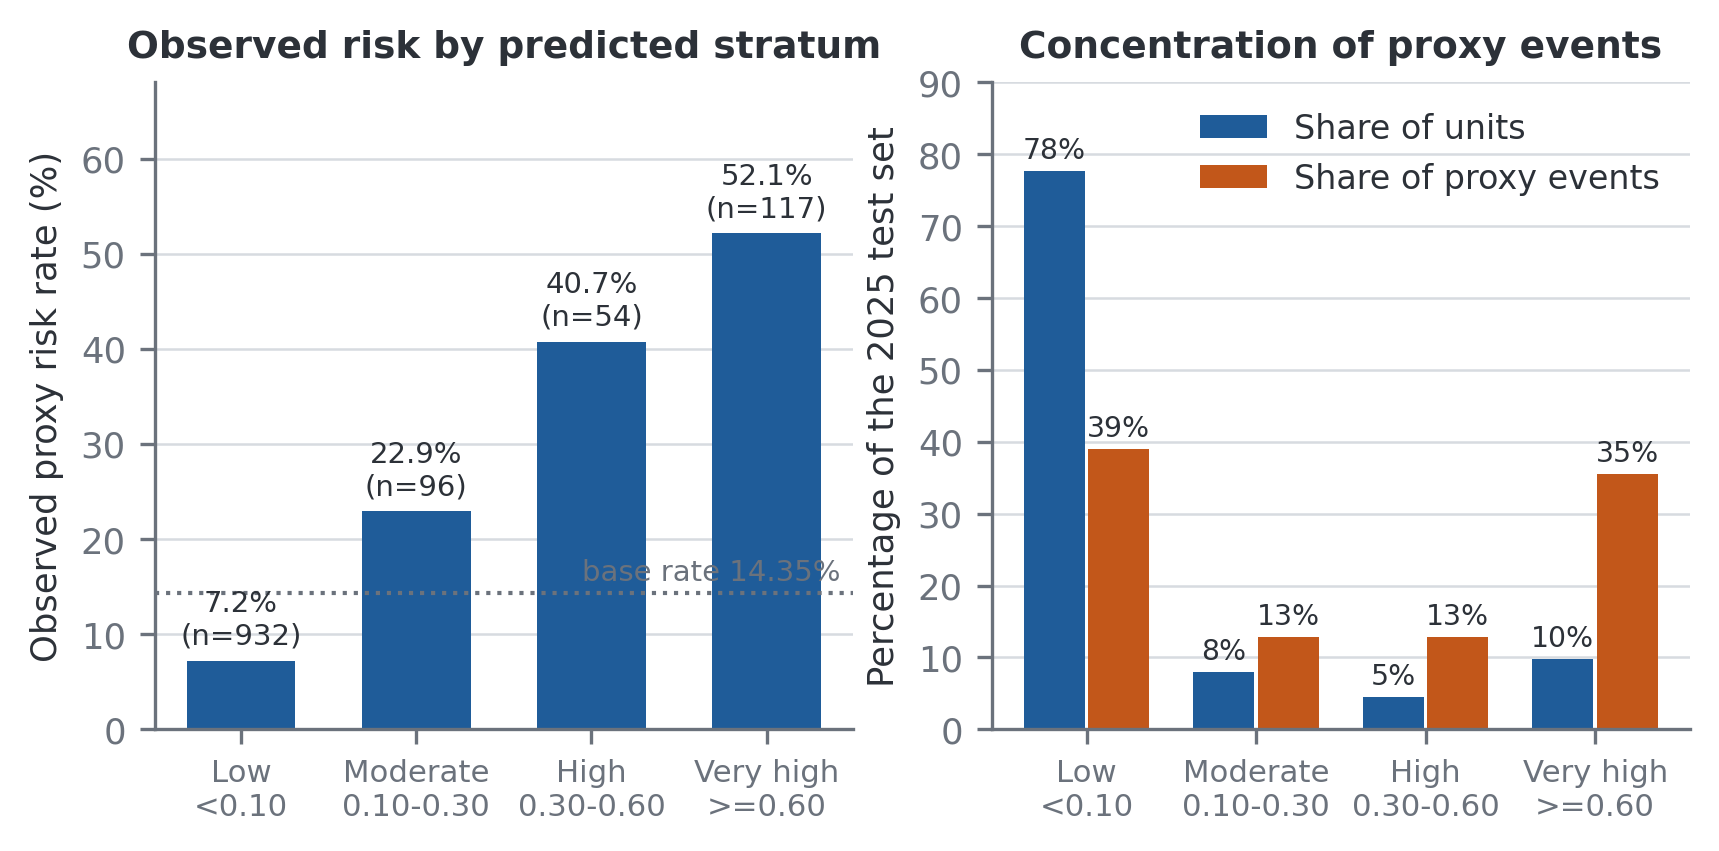
\includegraphics[width=0.98\textwidth]{figures/fig07_risk_strata.png}
\caption[Descriptive score strata on the 2025 evaluation set]{\textbf{Descriptive score strata on the 2025 evaluation set.} Left: observed overload rate by predicted stratum, against the base rate. Right: the share of operational units and of overload events falling in each stratum. Strata are fixed cut-offs of the uncalibrated predicted probability at 0.10, 0.30 and 0.60.}\label{fig:strata}
\end{figure}

Two qualifications are essential. First, these boundaries are defined on the uncalibrated probability scale characterised in Section~\ref{sec:calibration}; the mean predicted probability in the highest band is 0.807 against an observed rate of 0.521, so the band labels describe rank position, not risk magnitude. Second, the strata are derived from the same 2025 partition on which they are described. An independent validation of the boundaries on a data set not used to construct them has not been performed, and until it is, the stratification should be read as a description of the model's ranking behaviour rather than as a validated triage instrument.

\subsection{Decision-analytic utility}\label{sec:dca}

Discrimination and stratification say nothing about whether acting on the model is better than the alternatives available to a decision maker. Figure~\ref{fig:dca} and Table~\ref{tab:dca} apply Equation~\ref{eq:nb} across the range of threshold probabilities and compare the model against flagging every unit and flagging none.

\begin{table}[h]
\caption{Net benefit on the 2025 evaluation set}\label{tab:dca}
\begin{tabular}{lrrrrrl}
\toprule
$p_t$ & Units flagged & TP & FP & Model & Flag all & Preferred strategy \\
\midrule
0.10 & 267 & 105 & 162 & $+0.073$ & $+0.048$ & Model \\
0.20 & 203 & 90 & 113 & $+0.052$ & $-0.071$ & Model \\
0.30 & 171 & 83 & 88 & $+0.038$ & $-0.224$ & Model \\
0.40 & 155 & 77 & 78 & $+0.021$ & $-0.428$ & Model \\
0.50 & 134 & 70 & 64 & $+0.005$ & $-0.713$ & Model \\
\textbf{0.65} & \textbf{112} & \textbf{58} & \textbf{54} & $\mathbf{-0.035}$ & $-1.447$ & \textbf{Flag none} \\
0.70 & 99 & 53 & 46 & $-0.045$ & $-1.855$ & Flag none \\
0.80 & 89 & 50 & 39 & $-0.088$ & $-3.283$ & Flag none \\
0.90 & 55 & 29 & 26 & $-0.171$ & $-7.566$ & Flag none \\
\bottomrule
\end{tabular}
\footnotetext{The row in bold is the F1-optimal operating point adopted in Table~\ref{tab:final}. Flagging no unit yields a net benefit of zero by definition. Provenance differs between rows, and is stated here because it bounds their precision: the rows on the 0.10--0.90 grid are reconstructed from the fixed-width reliability bins of Table~\ref{tab:calibration}, so their true- and false-positive counts are integer-rounded bin aggregates, whereas the bolded row is computed from the exact confusion matrix at $\tau = 0.65$. The reconstructed grid should therefore be interpreted as an approximate representation of threshold-dependent utility, with the exact operating-point estimate at $\tau=0.65$ treated as the primary quantitative DCA result.}
\end{table}

\begin{figure}[h]
\centering
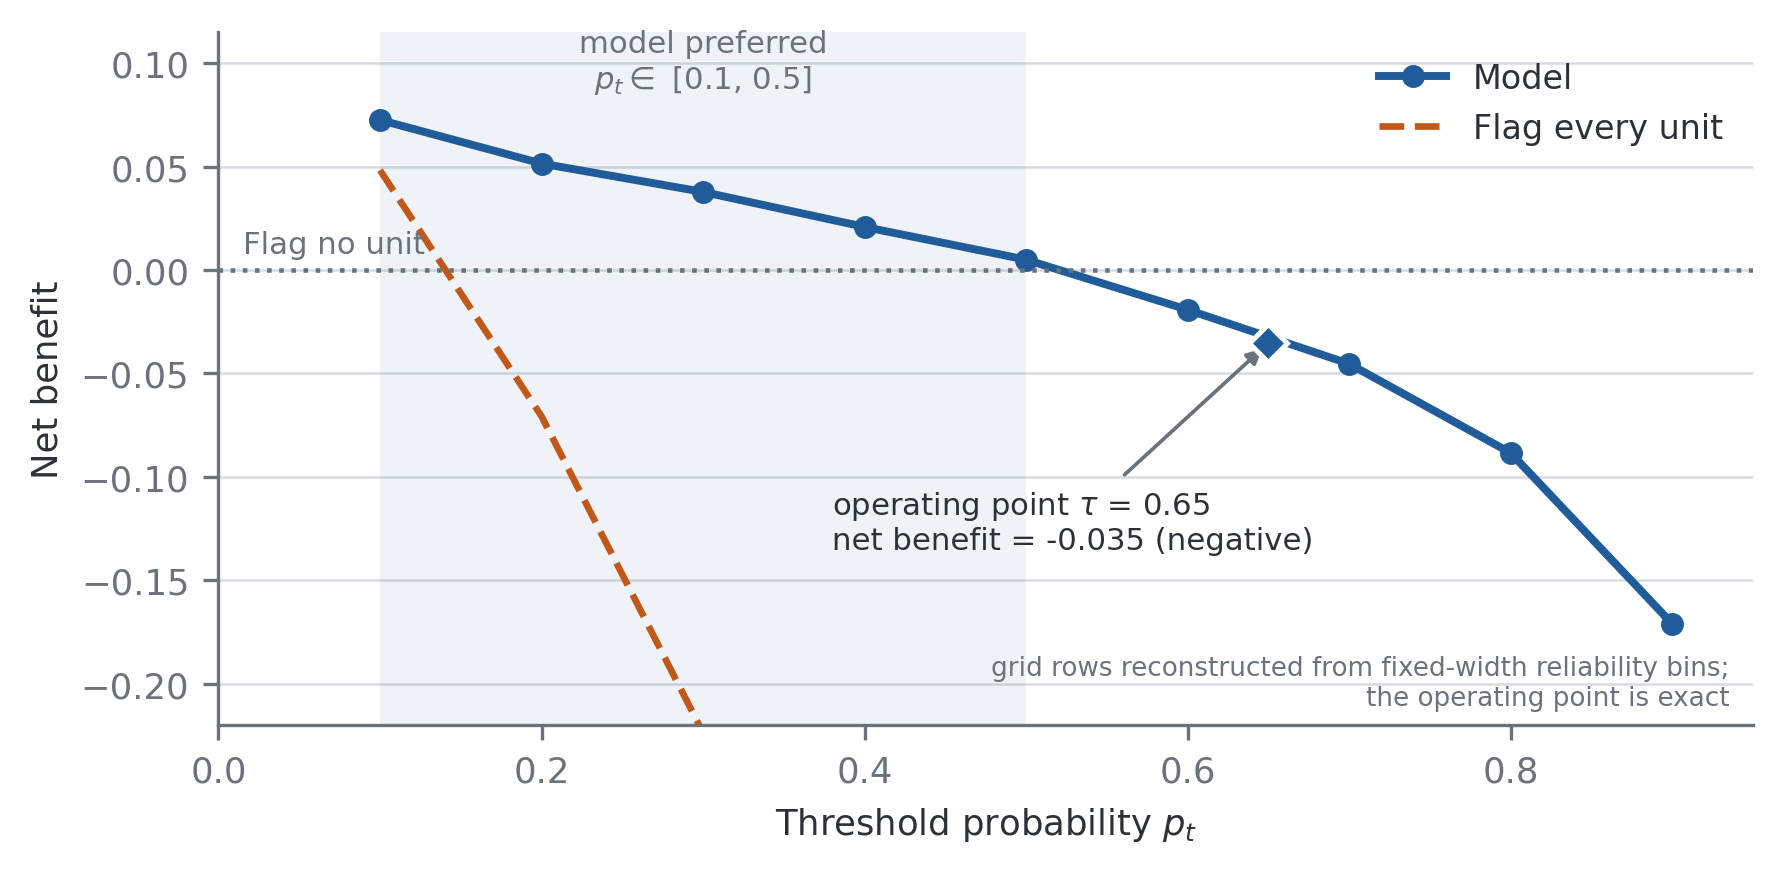
\includegraphics[width=0.92\textwidth]{figures/fig08_decision_curve.png}
\caption[Decision curve analysis on the 2025 evaluation set]{\textbf{Decision curve analysis on the 2025 evaluation set.} The model exceeds both default strategies for threshold probabilities between 0.1 and 0.5. At the F1-optimal operating point $\tau = 0.65$ its net benefit is negative, meaning that flagging no unit would be preferable for a decision maker holding that threshold. The grid is reconstructed from fixed-width reliability bins; only the operating point is computed from the exact confusion matrix.}\label{fig:dca}
\end{figure}

The result is deliberately interpreted conservatively, and the negative half of it is the more important. The reconstructed grid indicates positive net benefit for thresholds between approximately 0.1 and 0.5 and suggests dominance over the two reference policies in that range. But at the F1-optimal operating point of $\tau = 0.65$ --- the point at which the headline metrics of Table~\ref{tab:final} are computed --- the net benefit is $-0.035$. It is negative, and it is below the net benefit of the treat-none strategy. A decision maker who genuinely required a 65\% probability of overload before committing resources would be better off intervening nowhere than following this model's recommendations.

We draw the conclusion this requires. The threshold that optimises F1 is not a threshold at which the model is clinically useful, and the two criteria are not interchangeable. The framework supports the identification and ranking of units for review under moderate intervention costs, that is, for decision makers whose indifference threshold lies between roughly 0.1 and 0.5; it does not support a high-confidence alerting system, and we make no claim of operational utility at the F1-optimal operating point. This also reframes the illustrative cost calculation that a naive reading of the confusion matrix would invite: with 114 false negatives and 54 false positives, any monetary figure depends entirely on the assumed cost ratio, and the net benefit analysis is the principled way to express that dependence.

\subsection{Which variables drive the predictions}

Permutation importance computed on the reported XGBoost model and mean absolute SHAP values \cite{lundberg_unified_2017} computed on the tuned LightGBM configuration are shown in Figure~\ref{fig:importance}. We report both, and we label which model each was computed on, because the two attribution methods were applied to different estimators and are therefore not interchangeable; the agreement between them is a property worth reporting, not an assumption to be made silently.

\begin{figure}[h]
\centering
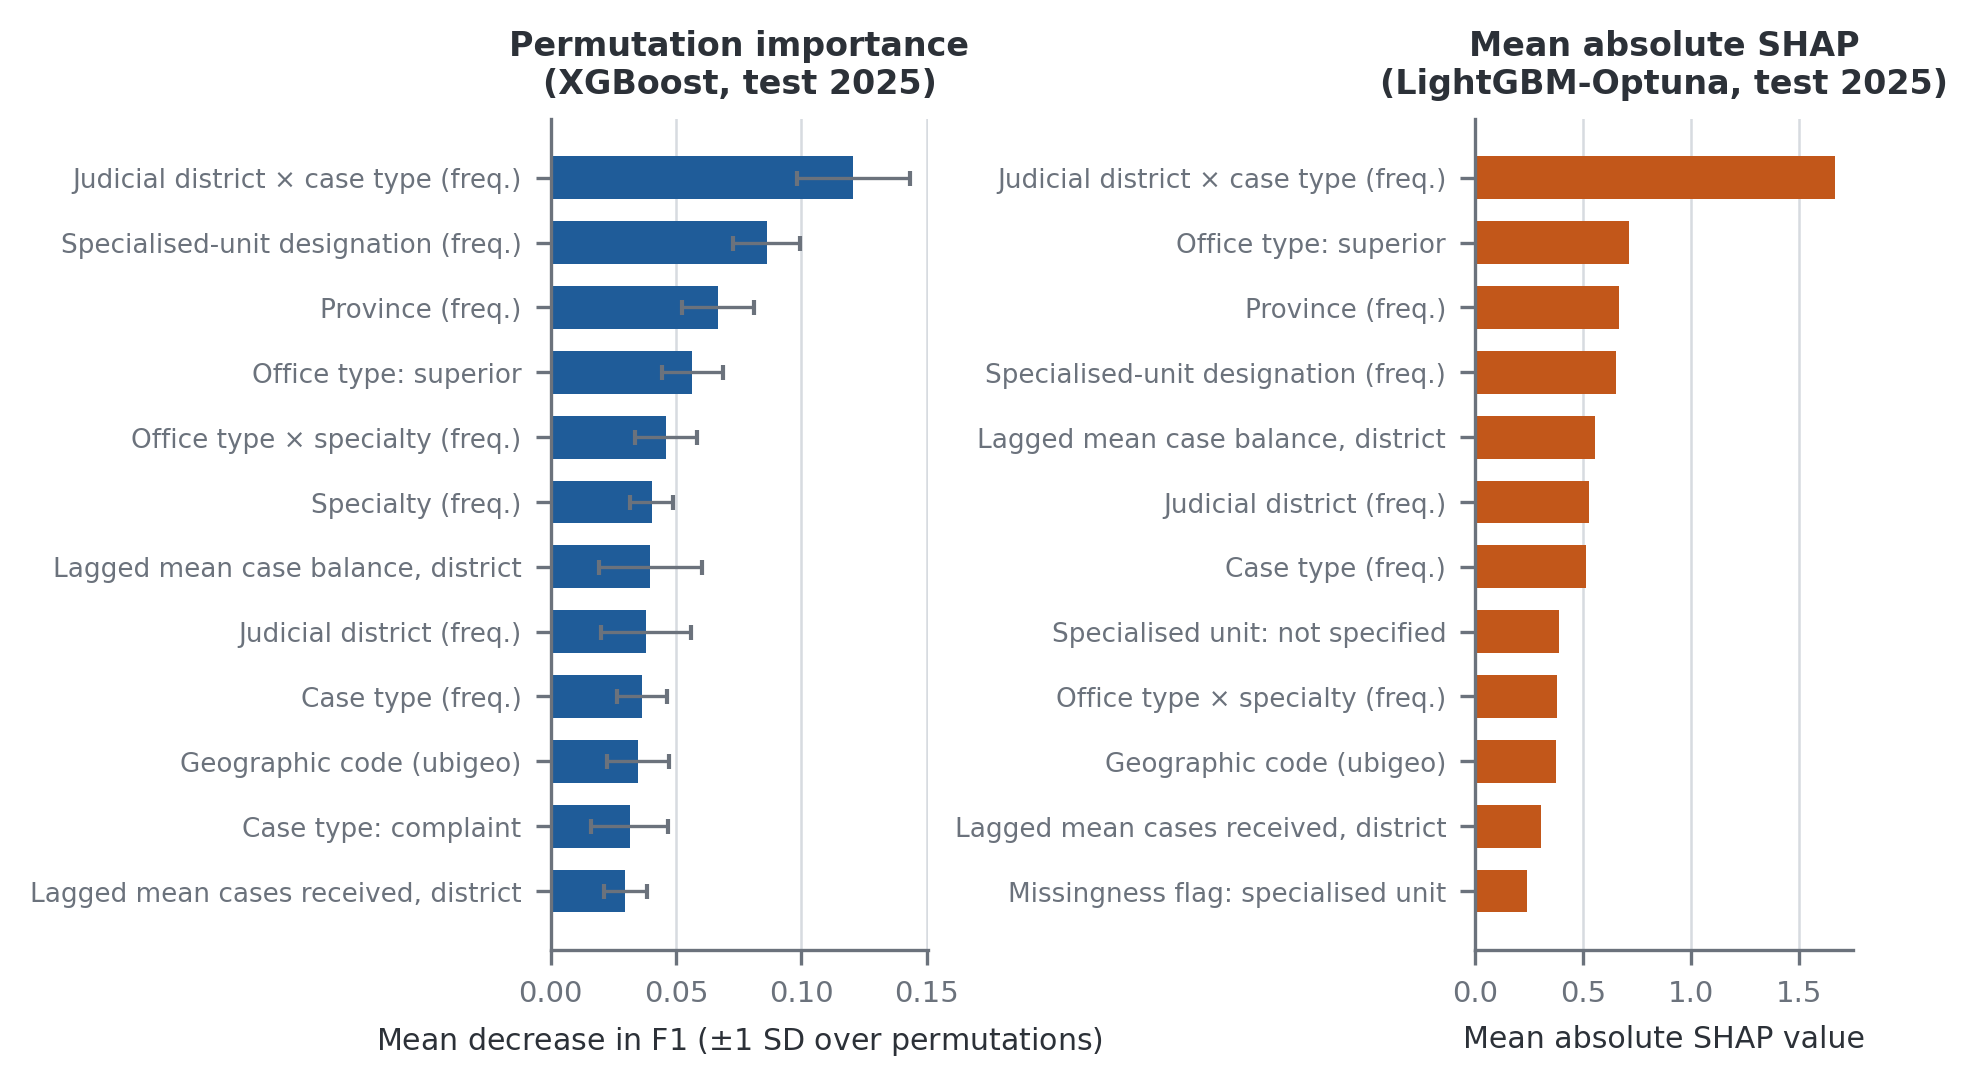
\includegraphics[width=0.98\textwidth]{figures/fig09_importance.png}
\caption[Global variable importance under two attribution methods]{\textbf{Global variable importance under two attribution methods.} Left: permutation importance on the reported XGBoost model, with error bars giving $\pm$1 SD over permutations. Right: mean absolute SHAP values on the tuned LightGBM configuration. The two attributions were computed on different estimators and are shown separately for that reason. Variables carry readable labels; Additional file~3 maps each label to the exact column name in the pipeline.}\label{fig:importance}
\end{figure}

In both evaluations, the primary contribution corresponds to the frequency encoding of the judicial district $\times$ case type interaction (permutation importance: 0.121; mean $\vert{}$SHAP$\vert{}$: 1.668), followed by the frequency of the specialized-unit designation, the frequency of the province, and the indicator for upper-tier prosecution offices. The lagged historical aggregates appear in the mid-range of both rankings. The two attribution analyses are directionally consistent in highlighting structural characteristics of the operational unit. Because the reported XGBoost model retains the three residual publication-metadata indicators described in Section~\ref{sec:availability}, this interpretation should be understood primarily as a description of the dominant structural predictors rather than as evidence that all reported model behaviour arises exclusively from admissible ex ante information.

The ablation study (Figure~\ref{fig:ablation}) supports this reading and delivers one counter-intuitive result. Each variant refits a single untuned LightGBM classifier (250 trees, learning rate 0.05, balanced class weights) on the corresponding feature subset, so the ablation measures the marginal contribution of each block under a common learner rather than the behaviour of the reported XGBoost configuration. The two are not interchangeable: the full-feature reference for the ablation is an F1 of 0.468, against the 0.458 that XGBoost attains at the same threshold in Table~\ref{tab:models}. Within that common learner, removing the territorial block costs 0.053 F1, the largest degradation of any single block. Removing the frequency encodings or the categorical interactions produces smaller changes. Removing the historical and growth block, however, \emph{improves} F1 by 0.031 and ROC-AUC by 0.026. Within this secondary LightGBM experiment, the lagged aggregates do not improve predictive performance on the locked evaluation set. This observation should not be interpreted as evidence that the same block is detrimental to the reported XGBoost configuration.

We report this rather than suppress it, with two qualifications attached. It is a LightGBM result, and whether it transfers to the reported model has not been tested. And it is computed on the locked partition, so it describes the feature set rather than justifying it; acting on it would require re-deriving the selection on the training block.

\begin{figure}[h]
\centering
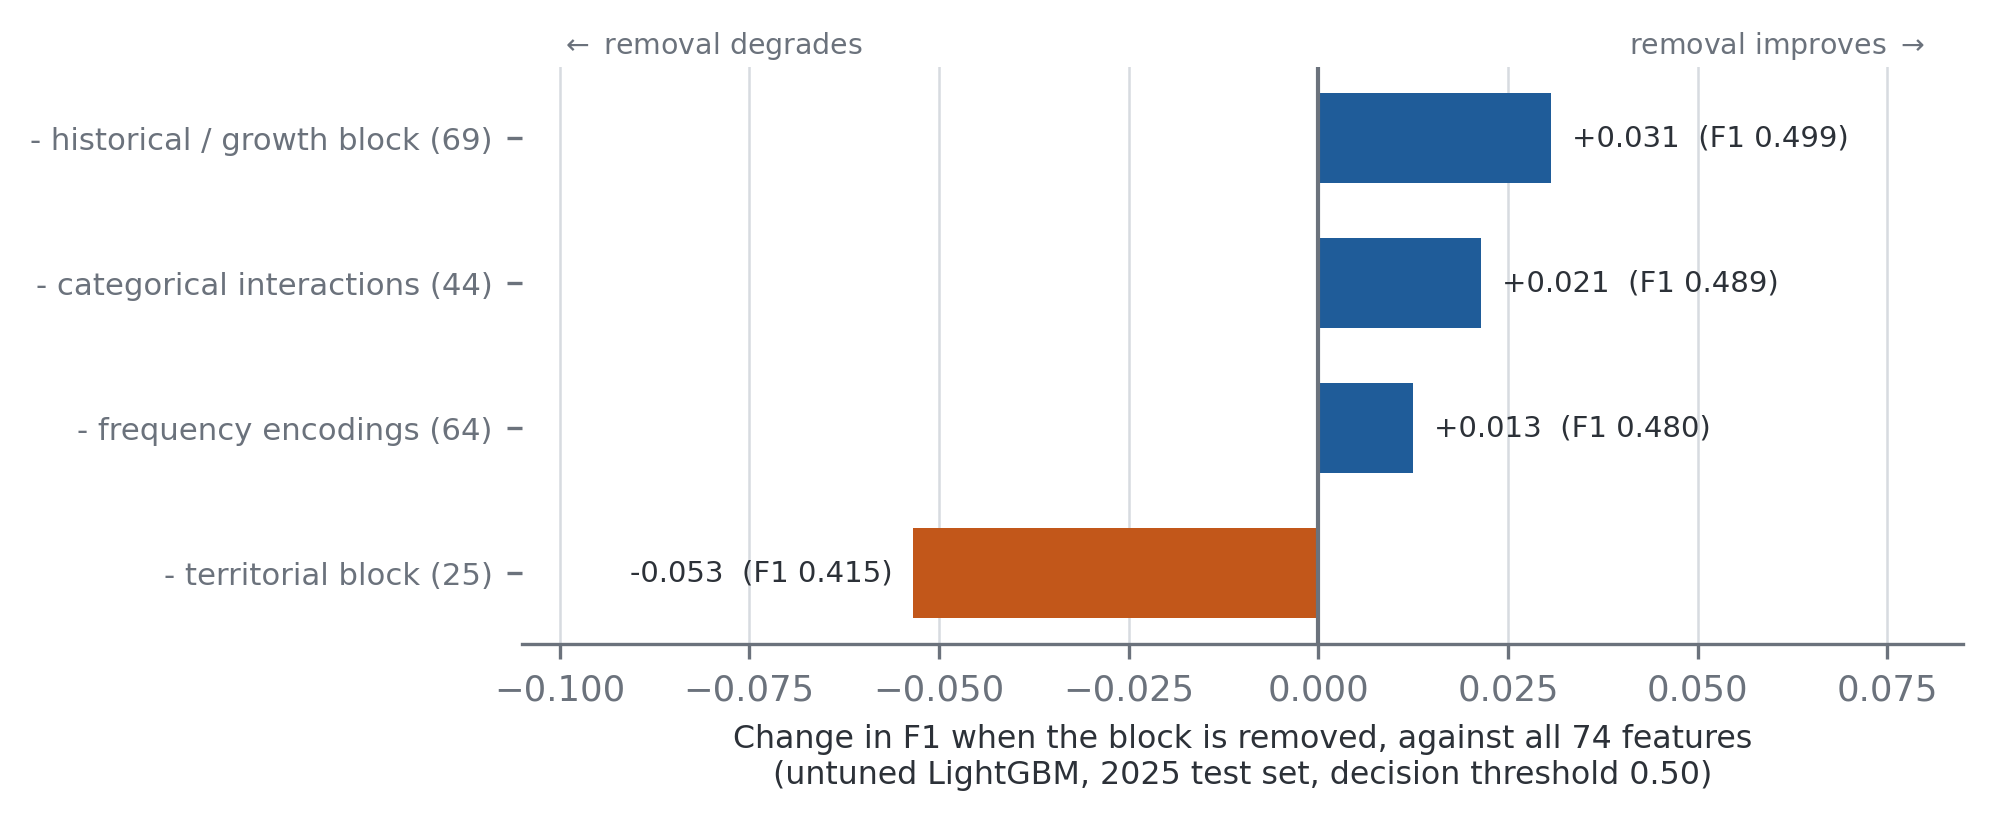
\includegraphics[width=0.90\textwidth]{figures/fig10_ablation.png}
\caption[Feature-block ablation on the 2025 evaluation set]{\textbf{Feature-block ablation on the 2025 evaluation set.} Bars give the change in F1 when a block is removed, against the full set of 74 features; the absolute F1 of each variant is printed beside its bar. Each variant refits an untuned LightGBM classifier on the corresponding subset and is evaluated at the reference threshold of 0.50, so the estimator differs from the reported XGBoost configuration and the full-set reference is 0.468 rather than 0.458. Removing the territorial block degrades performance most; removing the historical and growth block improves it.}\label{fig:ablation}
\end{figure}

\subsection{Subgroup behaviour and uncertainty quantification}

Subgroup analysis by territory reveals a substantial disparity. In the Lima metropolitan area (258 units, observed prevalence 16.7\%) the model flags 22.1\% of units and attains a true positive rate of 0.535 with a false positive rate of 0.158. In the provinces (941 units, observed prevalence 13.7\%) it flags only 5.8\% of units, attaining a true positive rate of 0.271 with a false positive rate of 0.025. The equal-opportunity gap of 0.264 means that an overloaded provincial unit is roughly half as likely to be identified as an equivalently overloaded metropolitan one. Because the model relies heavily on frequency encodings, and metropolitan configurations are more frequent in the registry, this disparity is a predictable consequence of the feature design rather than an incidental artefact. Any institutional use of the framework would have to correct for it, for example by calibrating and thresholding within territorial strata.

Split-conformal prediction \cite{vovk_algorithmic_2005} calibrated on the 2024 partition at a nominal coverage of 90\% achieves 87.3\% empirical coverage on 2025 and 83.7\% on the partial 2026 file, with 97.1\% and 95.6\% singleton prediction sets respectively. A Mondrian variant conditioned on the operational cluster gives 87.6\% and 84.8\%. The shortfall against nominal coverage is not within sampling error in either year: the Wilson 95\% interval for the 2025 figure is 85.3--89.1\% and for the 2026 figure 81.4--85.7\%, and neither contains 0.90. The coverage shortfall is interpreted as evidence of limited transportability of the calibration assumption rather than as a discrepancy of the conformal procedure itself. Split conformal prediction provides its marginal guarantee under an exchangeability assumption that is weakened when a calibration year is followed by a distributionally different evaluation year. The larger shortfall in 2026 is therefore consistent with the temporal shift detected by the drift analysis. This agreement between the uncertainty audit and the distribution-shift audit is one of the methodological findings of the framework.

Unsupervised profiling with $k$-means on the same availability-audited feature space selects a two-cluster approach (silhouette 0.371). The smaller cluster (1{,}269 units) exhibits an overload rate of 23.9\% against 13.3\% in the larger one, and this ordering is preserved under all four label scenarios. That an unsupervised partition of the admissible predictors recovers the same risk ordering as the supervised label is consistent with the construct, but the support it provides is weaker than the point estimates suggest: the bootstrap adjusted Rand index of the partition is $0.798 \pm 0.404$, a standard deviation more than half the mean, so the two-cluster solution itself is not stable under resampling. We report the convergence as suggestive and decline to treat it as validation.

\section{Discussion}\label{sec:discussion}

\subsection{What the evidence supports}

The framework shows that a proxy signal of prosecutorial overload can be ranked with predominantly structural predictors together with a small residual set of publication-metadata indicators intended to be available before the reporting year opens. On the locked 2025 evaluation, the reference configuration attains a ROC-AUC near 0.80, while the temporal analyses indicate that discrimination is reasonably stable across the complete-year walk-forward folds. However, this evidence must be interpreted together with the residual availability exposure documented in Section~\ref{sec:availability}.

\subsection{What the evidence does not support}

Three findings limit the claims that can be made, and they are stated here rather than buried.

The raw model scores should not be interpreted as calibrated risk estimates. Above a predicted probability of 0.3 they systematically over-estimate the observed rate, by as much as 0.46 in absolute terms. Any use that treats the output as an expected frequency --- resource allocation proportional to predicted risk, for example --- would over-allocate to the highest-scoring units.

At its own F1-optimal threshold the model has negative net benefit. This is the sharpest constraint, and it follows directly from the miscalibration: the threshold that maximises the harmonic mean of precision and recall lies in the region where the model's confidence is least warranted. Optimising a threshold for F1 and then presenting the result as evidence of operational value can be misleading that the decision curve analysis of Section~\ref{sec:dca} makes visible, and one that would have passed unnoticed had we reported discrimination alone.

The territorial disparity is large enough to matter. A framework whose sensitivity in the provinces is half its sensitivity in the capital cannot be deployed as an equitable prioritisation tool without stratified correction.

\subsection{Methodological implications of the audit}

The central methodological implication is that temporal leakage control should be treated as a property of the final fitted representation rather than solely as a preprocessing rule. In the present study, the initial availability classification correctly identified publication metadata as inadmissible, yet three derived indicators survived the subsequent feature-selection stage. Their absence from the evaluation years mitigate a direct inflation of the reported test figures, but their presence during training nevertheless allowed the estimator to encode year-specific information that would not be available at deployment. This distinction would remain invisible under a conventional train--test audit that checks only whether the evaluation rows are temporally separated.

The finding motivates a general protocol for longitudinal administrative machine learning: (i) define the prediction time point; (ii) classify every candidate variable by availability; (iii) restrict preprocessing and feature selection to information available within the training window; and (iv) repeat the availability audit on the final feature matrix immediately before model fitting. The fourth step is the principal methodological lesson of this case study. It provides a practical control against leakage introduced indirectly through feature engineering, encoding, metadata-derived variables or selection procedures.

\subsection{Interpreting the gap to the single-indicator rules}

The most instructive comparison in Table~\ref{tab:models} is between the learned models and the two rules that threshold the outcome year's own volumes. The rules reach F1 scores near 0.70; the models reach 0.46. That gap should not be interpreted solely as a deficiency of the learned models. It also quantifies the information penalty imposed by a genuinely ex ante prediction protocol.

In a study without such an audit, the volumetric variables would very likely have entered the feature set, the reported F1 would have approached 0.70, and the resulting figure would have described a model that cannot be run at the moment its prediction is needed. We regard the explicit reporting of both numbers, with the reason for the gap, as more useful than either number alone.

\subsection{Practical implications}

Read conservatively, the framework supports, at most, a review-prioritisation workflow: rank operational units by predicted score, direct planning attention to the upper strata, and use the conformal prediction sets to identify units for which the model declines to commit. Such use should be understood as decision support for human review rather than as an automated institutional decision rule. It does not support automated alerting, resource allocation proportional to predicted probability, or any decision requiring a high confidence threshold. Before institutional deployment, three steps are required: recalibration of the probability scale on a partition reserved for that purpose, re-derivation and independent validation of the risk bands on the recalibrated scale, and territorially stratified thresholding to close the equal-opportunity gap.

\section{Limitations}\label{sec:limits}

The label is a proxy constructed from a quantile rule, not an official certification of congestion; a unit flagged by this framework has a high case balance and a low processing rate, which is a plausible but not authoritative indicator of institutional overload. The evidence offered for it is an internal consistency check and a convergence with an unsupervised partition that is itself unstable under bootstrap; no expert panel was convened, and a formal Delphi or analytic hierarchy process elicitation remains outstanding. Up to 26 of the labels are additionally derived in part from an imputed processed-case count.

The reported model also retains the three publication-metadata indicators identified in Section~\ref{sec:availability}. Because the three indicators are identically zero throughout 2024--2026, they cannot contribute directly through non-zero values at evaluation time. However, their presence during training may have influenced the fitted model structure, so the possibility of residual indirect residual feature alignment cannot be ruled out without refitting the model after their removal.

The decision curve analysis is reported on a grid of threshold probabilities in steps of 0.10, reconstructed from the fixed-width reliability bins of the 2025 evaluation set rather than from per-record predicted probabilities; only the F1-optimal operating point is computed exactly, from the confusion matrix. Two consequences follow. The grid cannot resolve the crossing between the model and the treat-none strategy more finely than the interval 0.50--0.60, and the true- and false-positive counts along the grid are integer-rounded bin aggregates. Neither affects the sign of the net benefit at the reported operating point, which is exact, but recomputing the whole curve from per-record probabilities remains a straightforward outstanding step.

Two further quantities are reported at lower precision than would be ideal. The bootstrap confidence intervals of Table~\ref{tab:final} rest on 300 resamples, which is at the low end for a 95\% interval, and the maximum calibration error is attained in a reliability bin holding ten units. Both are recomputable from the per-record predictions of the frozen configuration without refitting any model.

Finally, the ablation of Section~\ref{sec:results} was computed with a single untuned LightGBM classifier rather than with the reported XGBoost model, so its conclusion about the historical feature block has not been shown to transfer to the configuration on which every other result rests.

The unit of analysis is an annual aggregate, which bounds the temporal resolution of any prediction to one year and mitigate the framework from anticipating within-year dynamics. The registry records no information on staffing, budget, procedural complexity or case severity, all of which plausibly influence processing capacity; their absence is a substantive constraint on achievable performance, and the persistent learning-curve gap is consistent with it. The 2026 file is partial and its results are exploratory throughout.

Finally, the framework has been evaluated on a single national registry. Its transferability to other prosecution services, or to judicial systems with different administrative structures, remains an open question.

\section{Conclusions}\label{sec:conclusions}

This study presents an auditable temporal machine learning framework for longitudinal administrative records, evaluated through the prediction of a proxy signal of prosecutorial overload in Peru. The central contribution is methodological rather than algorithmic: the framework makes temporal information availability, partition roles, feature-selection timing, predictive calibration and decision utility explicit components of model evaluation.

The availability audit shows why this distinction matters. Concurrent variables that define the proxy outcome were excluded from the intended predictor set, and preprocessing and feature selection were restricted to the training period. A second audit of the final fitted matrix nevertheless identified three publication-metadata indicators that had survived feature selection. Although these indicators are zero throughout the evaluation years and therefore cannot directly inflate the reported test predictions, their presence during training represents residual temporal exposure. Rather than treating this as an implementation detail, the study uses it to establish a general methodological requirement: temporal availability must be verified against the feature matrix that is actually fitted, not inferred solely from the initial exclusion rule.

The temporal partition protocol keeps model development, operating-point selection, locked evaluation and exploratory temporal generalisation distinct. The reference XGBoost configuration achieves a ROC-AUC of 0.796 (95\% CI 0.760--0.838) on the locked 2025 evaluation, indicating moderate discrimination under the information constraints imposed by the framework. However, calibration analysis shows systematic over-estimation at higher predicted scores, and decision-curve analysis yields negative net benefit at the F1-optimal threshold. The conformal analysis further shows reduced empirical coverage on later years, consistent with the temporal distribution shift identified in the drift analysis.

These findings illustrate the principal methodological lesson of the study: predictive discrimination, temporal validity, calibration, uncertainty and decision utility answer different questions and should not be collapsed into a single performance claim. A model may rank operational units reasonably well while still producing probabilities that are not calibrated, thresholds that do not provide positive decision utility, or uncertainty guarantees that weaken under temporal shift.

Accordingly, the framework should be interpreted as an auditable ranking and review-prioritisation procedure rather than as an automated alerting system. Before deployment, the strictly ex ante feature set must be re-derived and refitted, the probability scale and score strata must be independently recalibrated and validated, and territorial thresholding should be reconsidered in light of the observed equal-opportunity disparity.

More broadly, the study provides a reusable protocol and availability-audit template for longitudinal administrative machine learning. Its principal methodological proposition is simple but consequential: a model should not be considered temporally valid merely because its train and test rows are separated in time; the information content of the final fitted feature matrix must itself be auditable. The Peruvian prosecutorial registry provides the empirical setting in which this proposition is observed, while validation across other administrative domains remains an important direction for future work.

\backmatter

\section*{List of abbreviations}

\begin{description}
\item[ANOVA] Analysis of variance
\item[AUC] Area under the curve
\item[CI] Confidence interval
\item[CV] Cross-validation
\item[DCA] Decision curve analysis
\item[ECE] Expected calibration error
\item[MCC] Matthews correlation coefficient
\item[MCE] Maximum calibration error
\item[MPFN] Ministerio P\'ublico -- Fiscal\'ia de la Naci\'on (Public Prosecutor's Office of Peru)
\item[PR-AUC] Area under the precision--recall curve
\item[PSI] Population stability index
\item[RFE] Recursive feature elimination
\item[ROC-AUC] Area under the receiver operating characteristic curve
\item[SENATI] Servicio Nacional de Adiestramiento en Trabajo Industrial
\item[SHAP] SHapley Additive exPlanations
\item[SMOTE] Synthetic minority oversampling technique
\item[TRIPOD+AI] Transparent Reporting of a multivariable prediction model for Individual Prognosis Or Diagnosis, artificial intelligence extension
\end{description}

\section*{Declarations}

\begin{description}
\item[Ethics approval and consent to participate] Not applicable. The study uses publicly available aggregate administrative records released under an open data licence and involves no human subjects; no consent to participate was therefore required.
\item[Consent for publication] Not applicable.
\item[Availability of data and materials] The \emph{Casos Fiscales} data set analysed during the current study is publicly available from the Peruvian National Open Data Platform at \url{https://www.datosabiertos.gob.pe/dataset/mpfn-casos-fiscales} (accessed 25 August 2026). The complete analysis pipeline --- the availability audit, the partition protocol, the consensus selection and modelling stages, and the figure-generation scripts --- together with the derived result tables underlying every figure and table reported here, is available in the Zenodo repository, \emph{Source Code for Congestion Fiscal Research}, \url{https://doi.org/10.5281/zenodo.22118625} (accessed 26 August 2026), released under a Creative Commons Attribution 4.0 International licence. Additional file~1 contains the completed TRIPOD+AI reporting checklist; Additional file~2 contains the temporal availability audit template described in Section~\ref{sec:conclusions}; Additional file~3 maps the variable labels of Figure~\ref{fig:importance} to the column names used in the pipeline.
\item[Competing interests] The authors declare that they have no competing interests.
\item[Funding] No funding was received for this research.
\item[Authors' contributions] M.E.G. conceived the study, designed the methodology, implemented the pipeline and drafted the manuscript. J.A.C.L. contributed to the experimental design, the validation of results and the revision of the manuscript. Both authors read and approved the final version.
\item[Acknowledgements] We thank the Ministerio P\'ublico -- Fiscal\'ia de la Naci\'on of Peru for publishing the administrative records used in this study under an open data licence, and the anonymous reviewers whose comments on an earlier version motivated the availability audit, the partition protocol and the decision-analytic assessment reported here.
\end{description}

\bibliography{references}

\end{document}
